%\documentclass[pldi]{sigplanconf-pldi16}
%\documentclass[letterpaper,twocolumn,10pt]{article}
%\usepackage{usenix,epsfig,endnotes}

\documentclass[acmsmall,review,anonymous]{acmart}\settopmatter{printfolios=true,printccs=false,printacmref=false}





\settopmatter{printacmref=false} % Removes citation information below abstract
\renewcommand\footnotetextcopyrightpermission[1]{} % removes footnote with conference information in first column
\pagestyle{fancy} % removes running headers
% standard LaTeX packages
%\usepackage{changebar}

\usepackage{balance}
\usepackage{alltt}
\usepackage{amsmath}
\usepackage{balance}
\usepackage{booktabs}
\usepackage{fixltx2e}
\usepackage{graphicx}
\usepackage{boxedminipage}
\usepackage{hyperref}
\usepackage{nicefrac}
\usepackage{subfig}

\usepackage{setspace}
\usepackage{xspace}
\usepackage{multirow}
\usepackage{colortbl}
\usepackage{amsfonts} 
\usepackage{blindtext}
\usepackage{chngpage}
\usepackage{listings}
\usepackage{color}
\usepackage{natbib}
\usepackage{amssymb}% http://ctan.org/pkg/amssymb
\usepackage{pifont}% http://ctan.org/pkg/pifont
\bibliographystyle{abbrvnat}
\setcitestyle{authoryear,open={(},close={)}}



\captionsetup{format=default, font=bf}


\newcommand*{\Scale}[2][4]{\scalebox{#1}{$#2$}}%
\newcommand{\Tool}{ComAir\xspace}
\newcommand{\ComBugs}{30\xspace}
%\newcommand{\Code}[1]{\lstinline{#1}}
%\newcommand{\comment}[1]{{}}


\lstset{
  basicstyle=\tiny,
  columns=fullflexible,
  numbersep=5pt,
  numberstyle=\scriptsize,
  showstringspaces=false,
  escapeinside={/*@}{@*/},
  belowcaptionskip=1\baselineskip,
  language=C,
  showstringspaces=true,
  keywordstyle=\bfseries,
  commentstyle=\itshape,
}


\sloppy

\input macros.tex


\begin{document}





\title{Algorithmic Profiling for Real-World Complexity Problems}


\begin{abstract}
Complexity problems are one common type of performance problems, 
caused by algorithmic inefficiency. 
Algorithmic profiling aims to attribute complexity to a code construct.
It can detect previously unknown complexity problems and diagnose performance failures 
caused by complexity problems. 
Existing techniques on algorithmic profiling 
will incur more than $30$ times runtime overhead,
and cannot be deployed in production runs, missing opportunities to understand 
real-world workloads and how programs scale in the user side. 

In this paper, we present a toolchain \Tool, 
which can effectively conduct algorithmic profiling. 
To design \Tool, we first conduct an empirical study on 
real-world complexity problems from a representative performance-bug benchmark suit. 
Guided by our study, 
we then explore different 
design points during algorithmic profiling.
Finally, we apply sampling to lower runtime 
overhead and enable the production-run usage for \Tool.
Experimental results show that \Tool 
can cover different types of complexity problems, 
generate accurate profiling results, 
and incur a very low runtime overhead. 


\end{abstract}

\maketitle

\section{Introduction}
\label{sec:intro}

\subsection{Motivation}
\label{sec:motiv}

Performance problems~\footnote{We will use performance problems and performance bugs exchangeably, 
following previous works in this area~\cite{SongOOPSLA2014,ldoctor}} 
are one type of software implementation mistakes
and can cause inefficient execution~\cite{PerfBug,perf.fse10,SongOOPSLA2014,ldoctor,Alabama}. 
Performance problems cannot be optimized away by state-of-the-art compiler optimizations.
Due to the complexity of modern software and rapidly changing workloads, 
performance problems widely exist in production-run software, 
annoying end users and wasting energy in the field~\cite{PerfBug,SongOOPSLA2014,ldoctor}. 
Many highly-publicized failures have already been caused by performance problems, 
such as making a website costing millions of dollars useless~\cite{ACA-health}.
Combating performance problems is urgent. 

Many performance problems are caused by algorithmic inefficiency, 
such as implementing a linear algorithm in a $O(N^2)$ way.
We refer these performance problems as complexity problems in our paper.
Our empirical study on a representative performance-bug 
Benchmark set~\cite{PerfBug,SongOOPSLA2014} shows that 
nearly half user-perceived performance problems are complexity problems. 
Complexity problems are usually ranked high in developers' priority list. 
For example, Mozilla developers will immediately try to fix complexity bugs degrading exponentially~\cite{mozilla35294}. 
Addressing complexity problems is an important aspect to fight performance bugs. 


Algorithmic profiling~\cite{Aprof1,Aprof2,AlgoProf} collects profiles from multiple 
runs of the same program and attributes complexity to each code construct, like a loop or a function,
in the form of a \textit{cost} function of \textit{input} size. 
Algorithmic profiling can be used detect previously unknown complexity problems and 
diagnose performance failures caused by complexity problems. 

Algorithmic profiling is challenging. 
Effective techniques need to satisfy the following three requirements.
First, \textit{coverage}. Complexity problems are caused by a large variety of root causes. 
A code construct may take inputs and consume computation resources in various types.
A good technique must cover a large portion of various root causes, inputs and costs.
Second, \textit{accuracy}. Algorithmic profiling needs accurately identify 
how cost scales as input size changes.
Given an analyzed code construct,
it is desired to conduct algorithmic profiling under the context of the whole program's execution. 
Otherwise, missing how the code construct cooperate with other parts will lead to inaccurate results. 
Third, \textit{performance}. 
Developers' misunderstanding of real-world workloads 
is the most common reason why performance problems are introduced~\cite{PerfBug}. 
Production-run algorithmic profiling can help developers 
understand how their programs scale under these workloads.
However, production-run techniques require no observable slowdown from end users. 
For in-house testing, lowering runtime overhead can save testing time 
and allow developers to run more tests under a given time budget. 

Existing techniques do not satisfy the three conditions and 
cannot conduct algorithmic profiling effectively. 
Traditional profilers are most widely used tools to 
diagnose performance failure~\cite{gprof,oprofile}. 
Traditional profilers can only measure how much time spent in each code construct during one single run, 
while failing to connect information from multiple runs 
and failing to provide any indication about how execution time scales.
Therefore, traditional profilers fail in both coverage and accuracy.  
To understand asymptotic complexity for a code construct,
experimental algorithmics~\cite{expalg1,expalg2,expalg3} requires developers to 
extract the code construct and analyze it out of the original program. 
Although useful,
experimental algorithmics fail to consider how the code 
construct interact with the whole program and does not provide desired accuracy. 
Recent techniques on algorithmic profiling~\cite{Aprof1,Aprof2,AlgoProf} will incur more than 30X runtime overhead.
They cannot provide desired performance and are far from being deployed in production runs. 


\begin{figure}
\centering
\lstset{basicstyle=\ttfamily\fontsize{7}{8}\selectfont,
     morekeywords={+},keepspaces=true,numbers=left}
  \mbox{\lstinputlisting[mathescape,boxpos=t]{figure/mysql27287.c}}
\caption{A MySQL performance problem in polynomial complexity. 
\footnotesize{(During performance failure runs, 
   the total loop iterations scale polynomially in the size of \texttt{items}.)}}
\vspace{-0.05in}
\label{fig:mysql27287}
\vspace{-0.05in}
\end{figure}



\subsection{Contributions}
\label{sec:con}


Why we need algorithmic profiling? 

Why we need to push complexity profiling to production runs? 
a. Understanding real-world workload
b. Identifying performance bugs caused by API-misuse

The state of the art cannot be applied to production runs. 

To better understand real-world complexity problems,
we conduct an empirical study on complexity bugs 
in a representative performance bug benchmark suite~\cite{PerfBug,SongOOPSLA2014}.
To the best of our knowledge, our work is the first study focusing on complexity problems.
We divide studied complexity problems into different complexity categories.    
We study root causes, how user-perceived performance impact is generated, 
and fix strategies for each category.
We also investigate the reporting and diagnosis process for complexity problems. 
Our findings and implications can motivate future research on complexity problems. 
They already guide our design point selection when exploring in-house algorithmic profiling 
and inspire our approximate algorithms when building production-run techniques. 

After carefully studying the design points for in-house algorithmic profiling,
we started to build our in-house technique 
based on an existing algorithm~\cite{Aprof1,Aprof2} leveraging 
Read Memory Size (RMS) as input metric. 
We design 4 compiler and runtime optimizations 
to reduce the runtime overhead during algorithmic profiling.
Our optimizations can reduce instrumentation sites 
and can also accelerate instrumented hook functions. 
There are two scenarios where the existing algorithm fails to profile, 
which are recursive functions scaling as the value of input parameters 
and code constructs taking inputs from I/O.
We enhance the existing algorithm to address these two limitations. 




Specifically, we make the following contributions:

\begin{itemize}

\item First, we conduct the first empirical study on real-world complexity problems. 
We have several important findings and implications, including
1) around three fourths of studied complexity problems are 
caused by repeated executions of buggy code constructs,
such as loops or recursive functions;
2) for most complexity problems, 
users describe how to change input size to observe the scaling problem during reporting;
and 3) complexity problems usually take longer time to diagnose and fix, 
and more effective tool supports are needed.  

\item Second, we optimize and enhance an in-house algorithmic profiling algorithm.
Our proposed optimizations 
can reduce instrumentation sites and accelerate hook functions.
We augment the algorithm to handle two scenarios, 
where the existing version cannot profile correctly. 





\item Third, we propose two approximate algorithms to conduct algorithmic profiling in production runs. 

\end{itemize}


%\newpage
\section{Understanding Real-World Complexity Problems}
\label{sec:study}

In this section, we report an empirical study on real-world 
complexity problems. Our empirical study is conducted in two steps.

\begin{enumerate}

\item We build a taxonomy for the studied complexity bugs. 
For bugs in each category, 
we study what code constructs conduct the inefficient computation,
how the user-perceived slowdown is generated, 
and how to fix these bugs. 
Our studying results can help us 
make suitable design decisions when building \Tool. 

\item We investigate how these complexity problems are reported by end users
and how they are diagnosed by developers. 
This knowledge can help us understand what information is available from the user side
and help us understand the 
state of practice for combating complexity bugs.



\end{enumerate}

\subsection{Methodology}
\label{sec:meth}

%\begin{table}[h!]
\centering
\small
\begin{tabular}{|@{\hspace{3pt}}l@{\hspace{3pt}}|@{\hspace{3pt}}c@{\hspace{3pt}}|}
\hline
Application Suite Description (language) & \# of Bugs\\
\hline                            
{\bf Apache Suite} 	                    & 4\\
%\cline{1-1}
{HTTPD:	Web Server (C)	}& \\
{TomCat:  Web Application Server (Java)}& \\
{Ant:	Build management utility (Java)}& \\
%\hline
%JMeter	& Load test utility (Java) & \\
\hline                            
{\bf Chromium Suite} Google Chrome browser (C/C++) & 3\\
\hline
%\multicolumn{2}{|l|}
{\bf GCC Suite}  GCC \& G++ Compiler (C/C++)     & 8\\
\hline
{\bf Mozilla Suite}  & 10\\
%\cline{1-1}
{Firefox: Web Browser (C++, JavaScript)}& 	\\
{Thunderbird: Email Client (C++, JavaScript)}& \\
\hline
{\bf MySQL Suite}     & 5	\\
%\cline{1-1}
{Server: Database Server (C/C++)}&  	\\
%\cline{1}
{Connector: DB Client Libraries (C/C++/Java/.Net)} &  	\\
\hline
{\bf Total}	   & \ComBugs \\
\hline
\end{tabular}
\caption{Applications and complexity bugs used in the study.}
\label{tab:app_bug}
\end{table}

We conduct our empirical study based on a public benchmark set of 
real-world performance bugs~\cite{PerfBug,SongOOPSLA2014}. 
In their first work~\cite{PerfBug}, 
the authors collected 110 real-world performance bugs from 5 representative 
software suites: Apache, Chrome, GCC, Mozilla, and MySQL. 
%As shown in Figure~\ref{tab:app_bug}, 
These software suites cover various types of functionalities and are implemented 
in a variety of programming languages, including C/C++, Java, C\#, and JavaScript. 
All the five studied software suites are large and mature, 
with millions of lines of code and long development histories. 
In their following work~\cite{SongOOPSLA2014}, 
the authors further identified 65 user-perceived performance bugs, 
whose bugs reports contain detailed information 
about how these bugs are perceived by end users and fixed by developers.  

Our study focuses on user-perceived complexity bugs, 
because these bugs have large performance impact.
After carefully reading the bug reports and the buggy code fragments 
associated with these bugs,
we clearly identify \ComBugs performance problems 
caused by {\textit{algorithmic complexity}}.
Developers usually fix these bugs by applying optimized algorithms to lower complexity
or to reduce workloads processed by the buggy code fragments. 
We refer to these performance problems as 
{\textit{complexity problems}} in the reminder of this paper.
The number of the studied complexity problems is shown in Figure~\ref{tab:study}.
Bugs not belonging to complexity problems are caused by various reasons.
For example, there are several Mozilla bugs related to GUI, 
like drawing transparent figures or refreshing web pages too frequently. 
There are also bugs caused by misusing synchronizations, 
such as using busy wait or conducting I/O in a critical section. 
We do not consider these bugs as complexity problems.

{\bf{\textit{Caveats.}}}
In keeping with all previous empirical studies, 
our findings and conclusions need to be considered together with our methodology.
All of the studied complexity bugs come from software representative of a variety of uses and development processes. 
However, there are other types of software not covered in our study, 
such as distributed systems and software for high performance computation. 
All studied complexity problems are collected from bug databases.  
We believe that end users could report perceived complexity problems through other ways.
We also believe that there could be some complexity problems noticed 
and fixed by developers through manual inspection or in-house testing, 
before releasing their software to end users.  
%However, the field has not found methods to study bugs not tracked by bug databases.
We believe that the studied bugs can serve as a representative sample
of complexity problems in the real world. 



\subsection{A Taxonomy for Complexity Problems}
\label{sec:tax}


%\begin{table*}
%\begin{adjustwidth}{-.5in}{-.5in}
%\small
%\centering
%{
%\begin{tabular}{|lcccccc|}
%\hline
%                                                               &   Apache  &   Chrome   &  GCC   &    Mozilla   &   MySQL  &  Total\\
%\hline
%Total \# of complexity bugs                                          &   4       &    3       &   8    &    10        &   5      &   30 \\
%\hline
%\multicolumn{7}{|c|}{\bf Taxonomy of complexity problems}\\
%\multicolumn{1}{|l}{{\bf $O(N)$}: linear complexity}                 &   1       &    0       &   0    &    4         &   3      &   8\\
%\multicolumn{1}{|l}{{\bf $O(N^k)$}: polynomial complexity (k>1)}     &   3       &    3       &   5    &    6         &   1      &  18\\
%\multicolumn{1}{|l}{{\bf $O(e^N)$}: exponential complexity}          &   0       &    0       &   3    &    0         &   1      &   4\\
%\hline
%\multicolumn{7}{|c|}{\bf How complexity problems are reported?}\\
%\multicolumn{1}{|l}{How to change input size {\bf is} specified}     &  4&2&5&9&5&25\\
%\multicolumn{1}{|l}{How to change input size {\bf not} specified}    &  0&1&3&1&0&5\\
%\hline
%\end{tabular}
%}
%\end{adjustwidth}
%\caption{Categorization for Section~\ref{sec:study}.
%(This table shows how complexity problems distribute among different complexity categories
% and whether or not how to change input size is specified during reporing.)}
%\label{tab:study}
%\end{table*}


\begin{table*}[tb!]
\begin{adjustwidth}{-.5in}{-.5in}
\small
\centering
{
\begin{tabular}{|lcccccc|}
\hline
                                                                                  &   Apache  &   Chrome   &  GCC   &    Mozilla   &   MySQL  &  Total\\
\hline
Total \# of complexity bugs                                                       &   4       &    3       &   8    &    10        &   5      &   30 \\
\hline
\multicolumn{7}{|c|}{\bf Taxonomy of complexity problems}\\
\multicolumn{1}{|l}{{\bf $O(N)$}: linear complexity}                              &   1       &    0       &   0    &    4         &   2      &   7\\
\multicolumn{1}{|l}{{\bf $O(N^k)$}: polynomial complexity ($k>1$)}                &   3       &    3       &   5    &    6         &   2      &  19\\
\multicolumn{1}{|l}{{\bf $O(e^N)$}: exponential complexity}                       &   0       &    0       &   3    &    0         &   1      &   4\\
\hline
\multicolumn{7}{|c|}{\bf How complexity problems are fixed?}\\
\multicolumn{1}{|l}{Optimize {\bf directly}: Buggy code is revised}              &  3        &    3       &   4    &    9         &   5      &  24 \\
\multicolumn{1}{|l}{Optimize {\bf indirectly}: Workloads are skipped}              &  1        &    0       &   4    &    1         &   0      &   6\\
\hline
\multicolumn{7}{|c|}{\bf How complexity problems are reported?}\\
\multicolumn{1}{|l}{Input size {\bf is} specified}                                &  4        &    2       &   4    &    9    &5   &24\\
\multicolumn{1}{|l}{Input size is {\bf not} specified}                            &  0        &    1       &   4    &    1    &0   &6\\
\hline
\end{tabular}
}
\end{adjustwidth}
\caption{Categorization for Section~\ref{sec:study}.
\footnotesize{(This table shows how complexity problems distribute among different complexity categories, how developers fix studied complexity problems,
 and whether or not how to change input size is specified during reporting.)}}
\label{tab:study}
% \vspace{-0.4in}
\end{table*}


After categorizing the studied bugs according to their different complexity, 
we study complexity problems in each category.
Our study focuses on 
1) what are root causes\footnote{We refer root causes as code constructs 
conducting the inefficient computation, 
following previous works in this area~\cite{SongOOPSLA2014,ldoctor}.} 
of the complexity problems;
2) how the complexity problems generate user-perceived performance impact;
3) how developers fix these complexity problems. 

{\underline{\textit{$O(N)$: linear complexity.}}} 
As shown in Table~\ref{tab:study}, 
7 out of \ComBugs studied complexity problems are in linear complexity. 
All of these problems are caused by a buggy loop, 
whose average loop iteration number scales in terms of input size $N$.

Five of them are characterized by buggy loops that contain serialized I/O operations.
Users could perceive these bugs, 
even though the average loop iteration numbers are not large.
Patching these 5 bugs involves aggregating I/O operations 
or completely eliminating unnecessary I/O operations. 
For example, Mozilla\#490742 is caused by bookmarking 
tabs using individual database transactions. 
Even bookmarking 50 tabs can cause a timeout dialog 
window to pop up in a performance failure run. 
To fix this bug, Mozilla developers use one single aggregated transaction 
to bookmark all tabs.
As another example, Mozilla\#344059 is due to saving unchanged 
search engine preferences to SQLite, 
and it is fixed by saving search 
engine preferences only when some of them are changed.

For the other three bugs,
their buggy loops execute many iterations during performance failure runs.
They are fixed by adding shortcuts to completely skip the buggy loops. 
Taking MySQL\#33948 as an example,
MySQL developers followed a common practice to keep all table entries in the same linked list, 
including both used ones and free ones. 
The buggy loop iterates the linked list and looks for a free entry.
During performance failure runs, 
many table entries are used and the buggy loop must iterate excessively to find a free entry.
To fix this bug, MySQL developers simply separate used entries and free entries,
and keep them in two separated linked lists. 

To sum up, all of the $O(N)$ complexity problems are caused by a buggy loop. 
To fix them, developers directly optimize these loops or completely skip these loops. 


{\underline{\textit{$O(N^k)$: polynomial complexity (k>1).}}}
As shown in Table~\ref{tab:study}, 
more than half of the studied complexity bugs are in polynomial complexity. 
Similar to the complexity problems in linear complexity,
the polynomial complexity for each problem is also caused by a buggy loop.
However, {\bf both} of the loop execution number 
and the average loop iteration number
scale as input size $N$.


\begin{figure}
\centering
\lstset{basicstyle=\ttfamily\fontsize{7}{8}\selectfont,
     morekeywords={+},keepspaces=true,numbers=left}
  \mbox{\lstinputlisting[mathescape,boxpos=t]{figure/Mozilla477564.js}}
  \vspace{-0.1in}
\caption{A Mozilla complexity problem in $O(N^2)$ complexity.
\footnotesize{(This figure shows the buggy code fragment for Mozilla\#477564. 
The execution time scales polynomially with the number of nodes in a linked list.)}}
\vspace{-0.05in}
\label{fig:Mozilla477564}
\vspace{-0.15in}
\end{figure}

\begin{figure}
\centering
\lstset{basicstyle=\ttfamily\fontsize{7}{8}\selectfont,
     morekeywords={+},keepspaces=true,numbers=left}
  \mbox{\lstinputlisting[mathescape,boxpos=t]{figure/apache34464.c}}
  \vspace{-0.1in}
\caption{An Apache performance problem in $O(N^2)$ complexity and its patch. 
\footnotesize{(This figure shows the buggy code fragment for Apache\#34464. 
 The execution time scales polynomially with the number of characters read from \texttt{getchar()}.)}}
\vspace{-0.05in}
\label{fig:apache34464}
\vspace{-0.3in}
\end{figure}

\begin{figure*}
\centering
\subfloat[MySQL\#27287]{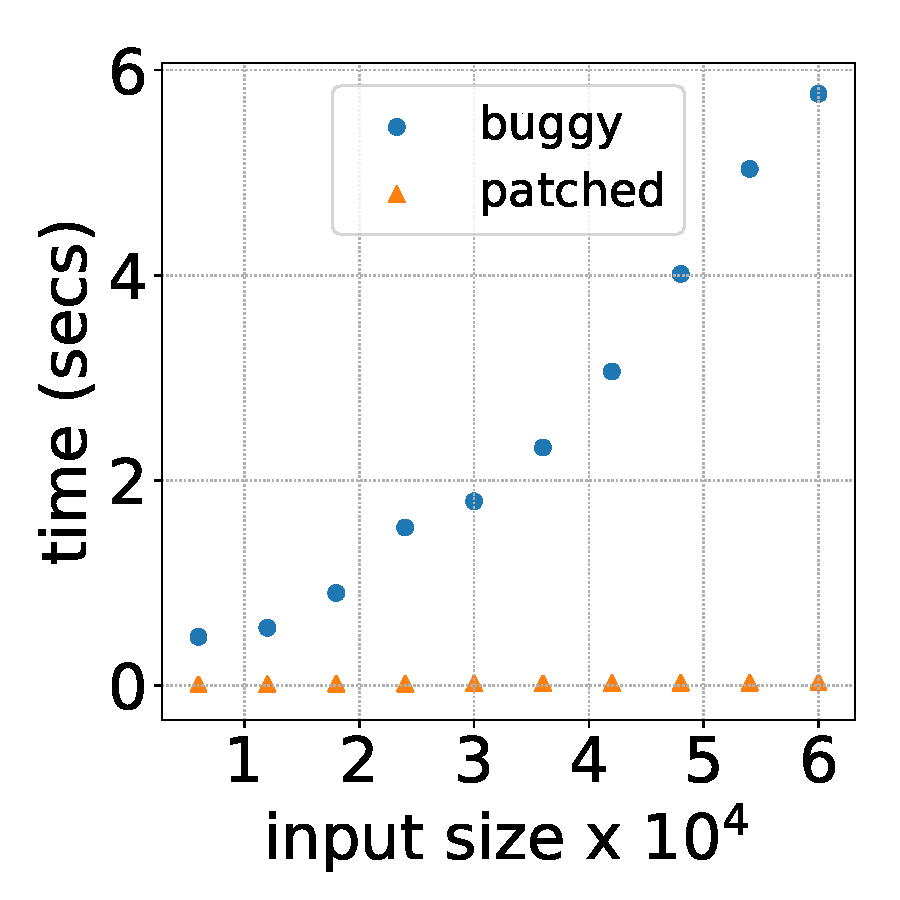
\includegraphics[width=0.22\linewidth]{figure/mysql27287-runtime-buggy-fixed-line}\label{fig:mysql27287-time}} 
\subfloat[Mozilla\#477564]{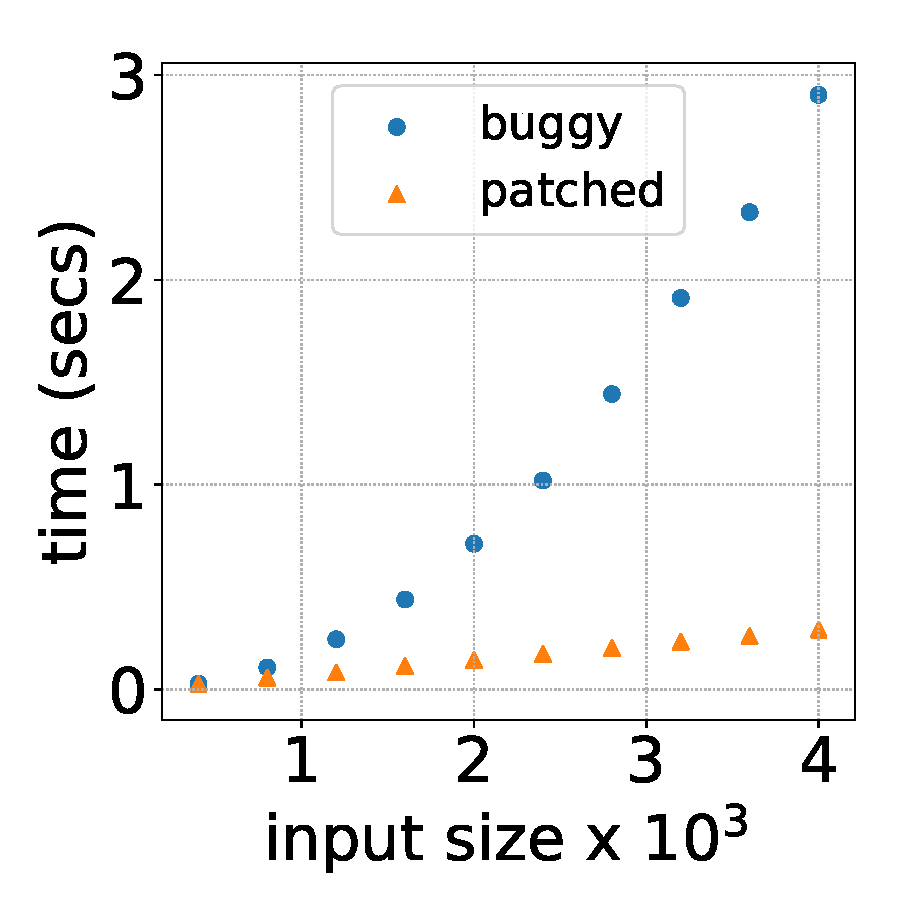
\includegraphics[width=0.22\linewidth]{figure/mozilla47564-runtime-buggy-fixed-line}\label{fig:mozilla477564-time}}
\subfloat[Apache\#34464]{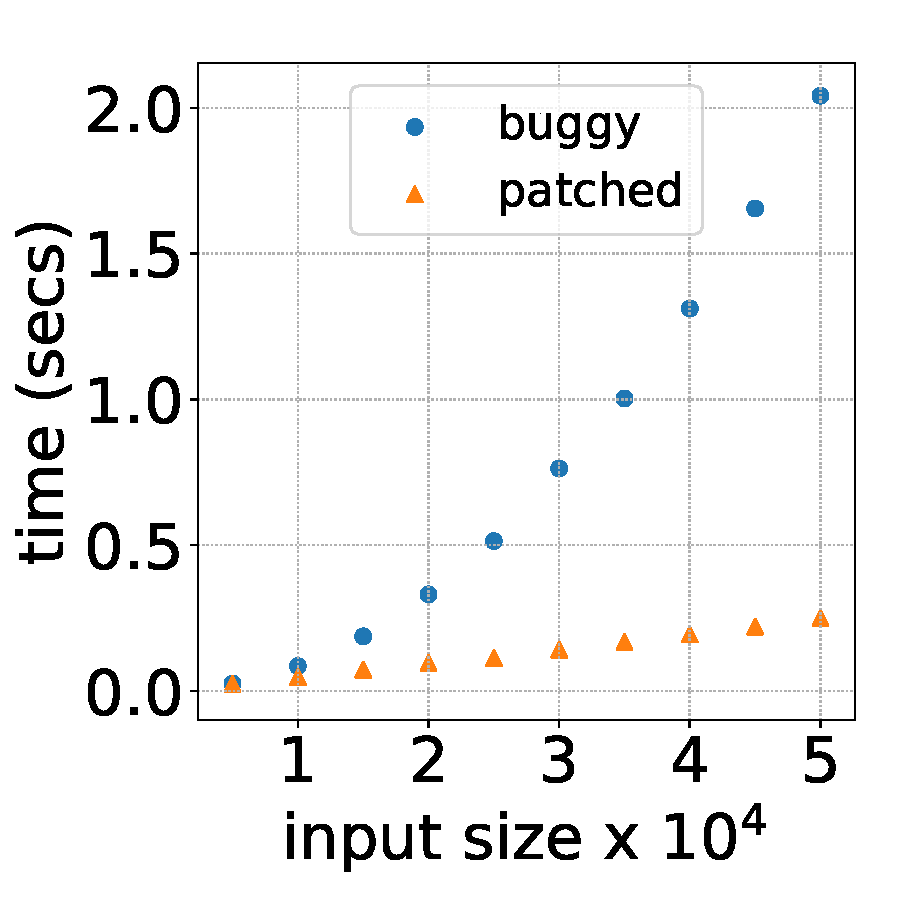
\includegraphics[width=0.22\linewidth]{figure/apache34464-runtime-buggy-fixed-line}\label{fig:apache34464-time}} 
\subfloat[GCC\#27733]{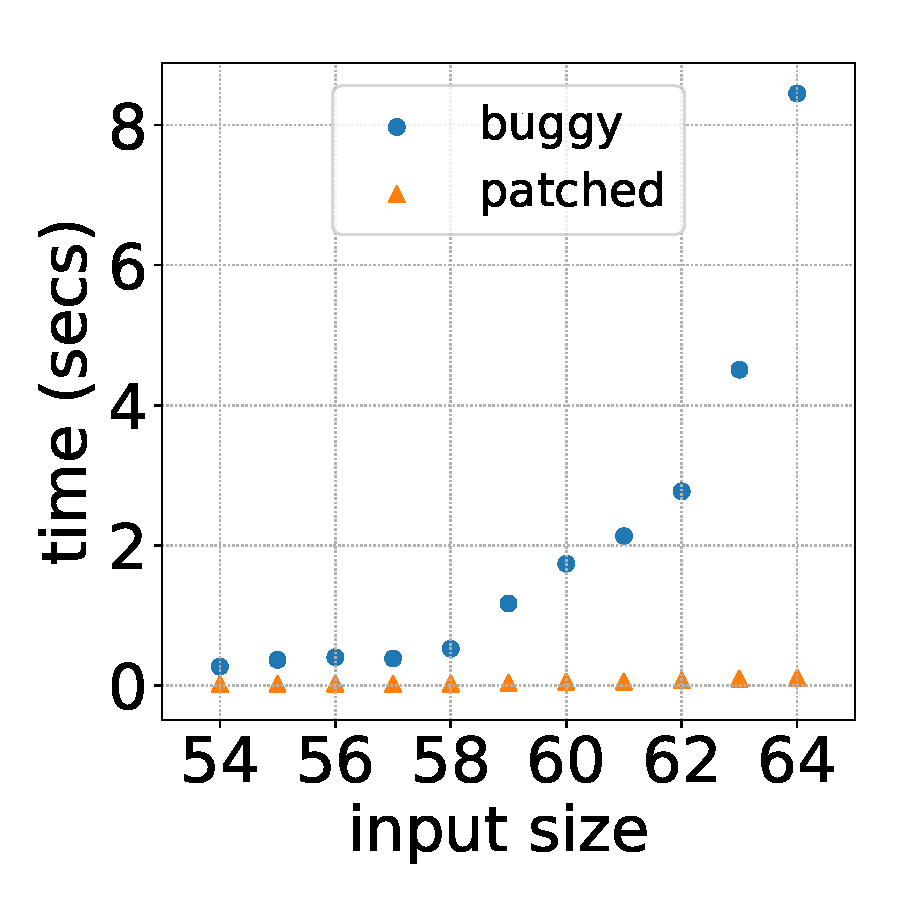
\includegraphics[width=0.22\linewidth]{figure/gcc27733-runtime-buggy-fixed-line}\label{fig:gcc27733-time}} \\ 
\vspace{-0.1in}
\caption{How the execution time scales with input size for four complexity problems. 
\footnotesize{(These figures show how the execution time changes with the change of input size for MySQL\#27287, 
 Apache\#34464, Mozilla\#477564, and GCC\#27733. For each complexity problem, we use 10 distinct inputs.)}} 
 \vspace{-0.05in}
\label{fig:time} 
\vspace{-0.15in}
\end{figure*} 

To fix the majority (14/19) of performance problems in this category,
developers directly modify the buggy loops, 
whose total iteration numbers scale polynomially.
Take MySQL\#27287 as an illustration.
As we discussed earlier, to fix this bug,
developers add an extra field to save parent \texttt{XML\_NODE}
and completely remove the buggy loop shown in Figure~\ref{fig:mysql27287}.
As another example, the buggy loop for Mozilla\#477564 is shown in Figure~\ref{fig:Mozilla477564}.
The loop counts how many previous nodes of input \texttt{aNode} 
having the same \texttt{localName} and \texttt{URI}.
An outer loop, not shown in the figure, 
will invoke \texttt{sss\_xph\_generate} for every node in a linked list, 
so that the complexity is $O(N^2)$ in terms of the number of nodes in the linked list.
To fix this complexity bug, developers add an extra field to each node to 
save the counting result. 
Given a node, 
its \texttt{count} value is calculated by adding one 
to the \texttt{count} value of 
its nearest previous node with the same \texttt{localName} and \texttt{URI}.  
How the complexity changes after patching for MySQL\#27287 and Mozilla\#477564 are 
shown in Figure~\ref{fig:mysql27287-time} and Figure~\ref{fig:mozilla477564-time}, respectively. 







%To fix the majority (13/18) of performance problems in this category, 
%developers directly modify the loops whose total loop iterations scale polynomially.  
%The buggy loop for MySQL\#27287 is shown in Figure~\ref{fig:mysql27287}.
%The loop searches parent \texttt{XML\_NODE} for function parameter \texttt{nitems}, 
%which presents array index for another \texttt{XML\_NODE}.
%All \texttt{XML\_NODE}s are maintained in array \texttt{items}. 
%The way the loop to conduct the search is to iterate array \texttt{items} 
%backward from the input and look for the first \texttt{XML\_NODE} 
%whose level is one less than the input.
%During performance failure runs, 
%one \texttt{XML\_NODE} contains tens of thousands of children, 
%and \texttt{xml\_parent\_tag} is invoked for each of its children. 
%To fix this bug, MySQL developers add an extra field to each 
%\texttt{XML\_NODE} to save its parent, 
%and this field is initialized when a \texttt{XML\_NODE} is created. 
%After that, the buggy loop is completely removed. 


To fix the other complexity problems (5/19) in this category,
developers reduce data processed by the loops scaling polynomially, 
instead of changing the loops directly.
In the buggy code fragment for Apache\#34464 shown in Figure~\ref{fig:apache34464},
the \texttt{while} loop on line 5 searches a string \texttt{source}
for a target sub-string \texttt{target}.
If the \texttt{while} loop's search is unsuccessful, 
a new character returned from \texttt{getchar()} on line 8 will be appended to string \texttt{source}, 
and the loop will search string \texttt{source} again from the beginning. 
There is an inner loop inside \texttt{indexOf()}, whose total iterations 
scale polynomially in terms of the number of characters from \texttt{getchar()}. 
After fixing this bug, the inner loop will only check the most recent \texttt{targetLen} characters.
The developers do not change the inner loop, 
while reducing the workload it processes.   
How execution time scales before and after patching for 
Apache\#34464 is shown in Figure~\ref{fig:apache34464-time}.


%Take GCC\#12322 as another example.
%The loop scaling polynomially is part of the functionality that does basic block reordering,
%and it will perform poorly for basic blocks with too many successors. 
%The bug-triggering input contains a basic block with thousands of successors. 
%To fix this, developers simply skip basic blocks with many successors.
%By does this, some optimization opportunities may be lost, 
%but the generated codes will still work correctly. 


{\underline{\textit{$O(e^N)$: exponential complexity.}}}
Four of the studied complexity problems are in exponential complexity. 
These complexity problems are fixed 
either by leveraging memoization to reuse previous results 
or by skipping the computation with exponential complexity for large workloads. 



\begin{figure}
\centering
\lstset{basicstyle=\ttfamily\fontsize{7}{8}\selectfont,
     morekeywords={+},keepspaces=true,numbers=left}
  \mbox{\lstinputlisting[mathescape,boxpos=t]{figure/gcc27733.c}}
  \vspace{-0.1in}
\caption{A GCC performance problem in exponential complexity. 
 \footnotesize{(During performance failure runs, how many times \texttt{mult\_alg} is invoked scales exponentially
  with the number of 1s in the binary form of input \texttt{t}.)}}
\vspace{-0.1in}
\label{fig:gcc27733}
\vspace{-0.15in}
\end{figure}


Three of the studied performance problems are caused by recursive function calls. 
Taking GCC\#27733 in Figure~\ref{fig:gcc27733} as an example, 
the recursive function \texttt{mult\_alg} computes the best algorithm to multiply \texttt{t}.
In each invocation, \texttt{mult\_alg} will try a set of bitwise 
operations to change input 
\texttt{t} into a smaller number, \texttt{t'}, 
and recursively call itself.
The number of times when \texttt{mult\_alg} is invoked scales exponentially 
in terms of the number of 1s in the binary form of input \texttt{t}.
To optimize this function, 
GCC developers use a hash table, \texttt{alg\_hash}, to record
which \texttt{t} has been processed before and its corresponding result.
However, there is a type declaration error inside the hash table entry,
and this error causes \texttt{t} larger than the maximum unsigned integer to never hit cache.
For large \texttt{t}, \texttt{mult\_alg} is still in exponential complexity. 
After fixing the type declaration error, 
memoization is enabled for large \texttt{t}. 
How the complexity changes after patching for GCC\#27733 is shown in Figure~\ref{fig:gcc27733-time}.

GCC\#32540 is in the exponential complexity category and is caused by an inefficient loop. 
The loop applies an iterative algorithm to implement a compiler optimization. 
The bug-triggering input contains very complex control and data dependence,  
so that the buggy loop scales exponentially in terms of the number 
of \texttt{if} branches in the input. 
To fix this bug, developers simply disable the optimization 
once they detect the complex control and data dependence.  


\subsection{Diagnosis process of complexity problems}
\label{sec:process}

We also study how complexity problems are reported by users 
and get diagnosed by developers 
to better understand state-of-the-art combating process for complexity problems. 

{\underline{\textit{How are complexity problems reported?}}
As shown in Table~\ref{tab:study},
for most complexity bugs (24/30), 
users' reports specify how to change input sizes 
in order to reproduce the performance scaling problems. 
As discussed in previous works~\cite{SongOOPSLA2014}, 
all collected user-perceived performance-bug reports
contain bug-triggering inputs from end users. 
For most complexity bugs, 
users also describe how they change input sizes 
and how performance changes accordingly. 
For example, when reporting GCC\#32540, 
the user provides a C file and several measurement results to 
show that GCC compilation time scales exponentially 
with the number of \texttt{if} branches in the C file. 
As another example, when reporting Mozilla\#490742, 
the user mentions that the length of high, 
flat CPU usage is related to the number of search engine preferences. 


For the other five bugs, users provide one bug-triggering input 
or describe a set of bug-triggering inputs when they report the complexity problems. 
For example, when reporting GCC\#27733, 
the user provides one bad input, which can take GCC 49 minutes to compile. 
When reporting Mozilla\#231300, the user mentions 
that clearing the disk cache on a Macintosh system can trigger the bug, 
regardless of the content of the cached files. 


{\underline{\textit{How complexity problems are diagnosed?}}
We studied how long it takes developers to fix complexity problems. 
On average, it takes developers 162 days to diagnose a complexity problem. 
Following the same methodology as the previous work~\cite{SongOOPSLA2014},
we calculate diagnosis time as starting from when a problem 
was reported to a bug tracking system
and ending when a correct patch was submitted on the bug tracking system. 
On average, it takes developers 101 days to diagnose non-complexity bugs in the same performance-bug set. 
Diagnosing complexity problems takes longer time.
After separating bugs from different applications, 
we also observe that developers consistently need more time to diagnose complexity problems across all applications.
%compared with non-complexity bugs.
%Among the five applications, 
%Chrome developers need 4.5 times longer to diagnose complexity problems,
%which is the maximum increase.
%MySQL developers spend most similar time to diagnose complexity problems,
%while the time they spend is still 0.43 times longer. 

As discussed in the previous works~\cite{SongOOPSLA2014}, 
traditional profilers are the only type of diagnosis tools mentioned in bug reports. 
%when diagnosing the collected user-perceived performance problems. 
Tradisional profilers are mentioned in 7 out of 30 complexity-bug reports. 
A similar percentage of bug reports mention traditional profilers
when comparing complexity bugs with non-complexity bugs. 

\subsection{Implications}
\label{sec:study_impli}

{\underline{\textit{Implication 1}}
The patches for most of the studied complexity problems (24/30)
are designed to directly optimize loops or recursive functions that scale poorly.
Accurately attributing complexity to loops or to functions can provide 
effective guidance for developers' investigation. 
Our study also shows that developers need to spend more time to 
diagnose and fix complexity problems.
Traditional profilers are the only type of tools 
mentioned during diagnosing complexity bugs, 
and traditional profilers can only tell where computation is spent in each run, 
while they are {\bf unable} to analyze or predict how computation scales across different runs.
To sum up, automated algorithmic profilers are 
uniquely needed to effectively combat complexity problems.  


{\underline{\textit{Implication 2}}
To effectively profile algorithmic complexity,
a set of inputs providing similar code coverage with different input sizes is needed. 
Our study shows that when reporting complexity problems,
users will describe how to change input sizes 
while preserving similar functionalities (or code coverage). 
This means it is fairly easy for developers to get the inputs needed 
to conduct diagnosis or algorithmic profiling for user-reported complexity problems. 

{\underline{\textit{Implication 3}}}
We also examine what types of data structures holding inputs processed 
by buggy loops or recursive functions for the studied complexity problems.
The most two common types of data structures 
are array (11/30) and linked list (9/30).
Other types of data structures are either application-specific or 
can only cover one or two bugs.
For example, the buggy recursive function for MySQL\#49047 is to detect deadlocks,
and the data structure holding inputs is a graph recording information about lock holding and lock requiring. 
Apache\#29743 is the only bug in our studied bug set 
whose buggy loop is to process a hash map. 
If we want to monitor workloads and conduct 
algorithmic profiling from the point of monitoring data structures, 
array and linked list are the two types of data structures 
we should start with.

{\underline{\textit{Implication 4}}
We also seek to understand how complexity problems are introduced. 
20 out of 30 studied complexity bugs are introduced
because the developers' workload assumptions are wrong or the workloads changed. 
This result motivates to monitor workloads and conduct algorithmic profiling in production runs. 
Workload monitoring tools can warn developers when the workload assumption is wrong.
Online algorithmic profiling tools can tell developers 
how each piece of code scales under real-world workloads on the user side.  

{\underline{\textit{Implication 5}}}
Our study shows that approximately three-fourths of the studied complexity problems (22/30)
are caused by repeated executions of a loop or a recursive function. 
These bugs are categorized as polynomial complexity and exponential complexity in Section~\ref{sec:tax}.
Previous works~\cite{SongOOPSLA2014,ldoctor} 
show that sampling code constructs 
that execute many times in one program run can lower the runtime overhead 
while preserving the same diagnosis or detection capability. 
It is promising to apply sampling to design production-run algorithmic profiling techniques. 


\newpage
\section{In-house Algorithmic Profiling}
\label{sec:inhouse}

In this section, we discuss the design and implementation for in-house algorithmic profiling.
Under in-house setting, 
developers can conduct algorithmic profiling 
to detect previously unknown complexity problems before releasing their software, 
or developers could diagnose and fix complexity problems 
reported by users through bug databases.
%For both of these two cases, 
%run-time overhead is not a major concern. 


\subsection{Design}
To conduct algorithmic profiling~\cite{Aprof1,Aprof2,AlgoProf},
we first need to record input \textit{size} and \textit{cost} for different code constructs 
during multiple executions,
we then plot records from the same code construct with input size as x-axis and cost as y-axis, 
and finally, we infer a cost function of the input size by using 
statistical curve fitting~\cite{curve-fitting} 
or curving bounding~\cite{curve-bounding}. 
Code constructs could be loops~\cite{AlgoProf} and functions~\cite{Aprof1,Aprof2}. 
To design algorithmic profiling, we need to select 
suitable metrics for input size and cost. 


%\begin{figure*}
%\centering
%\subfloat[MySQL\#27287]{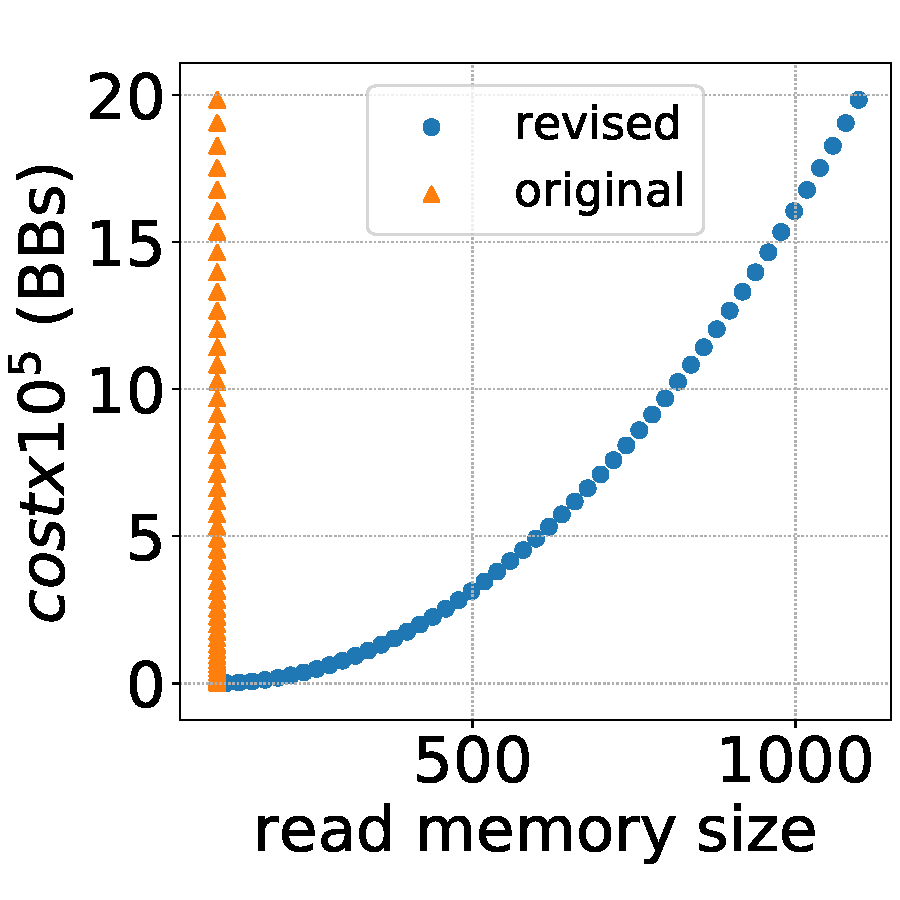
\includegraphics[width=0.24\linewidth]{figure/apache34464-line}\label{fig:mysql27287-line}} 
%\subfloat[GCC\#1687]{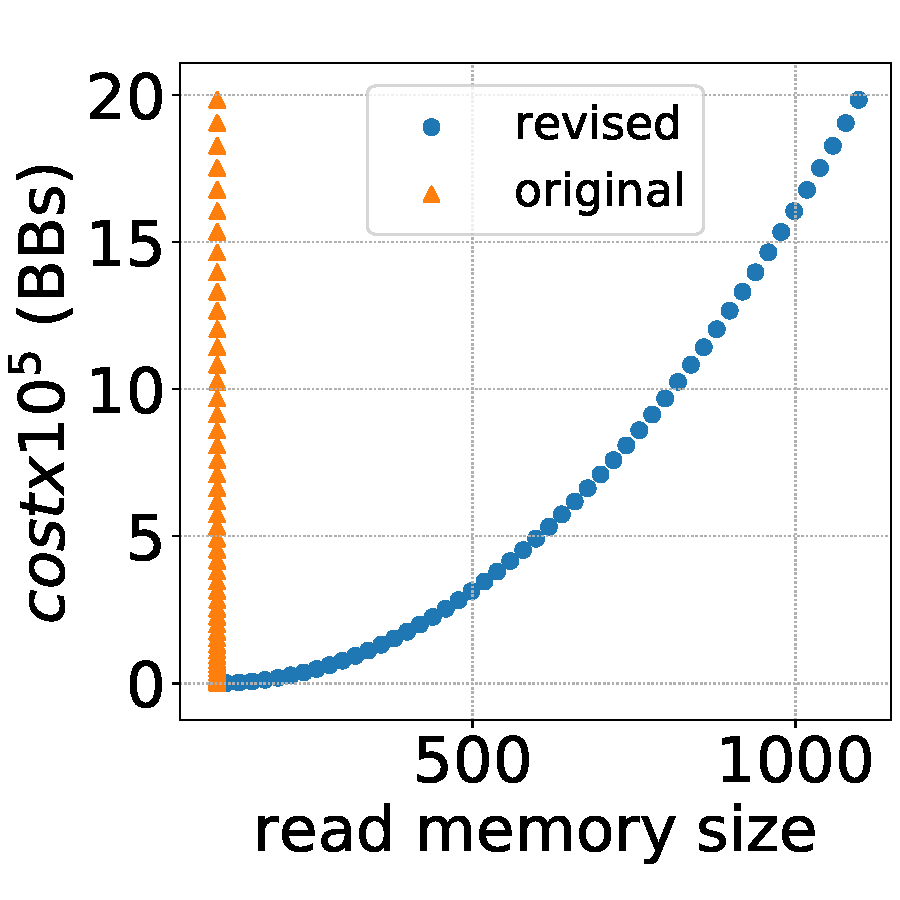
\includegraphics[width=0.24\linewidth]{figure/apache34464-line}\label{fig:jaccard}}
%\subfloat[fib]{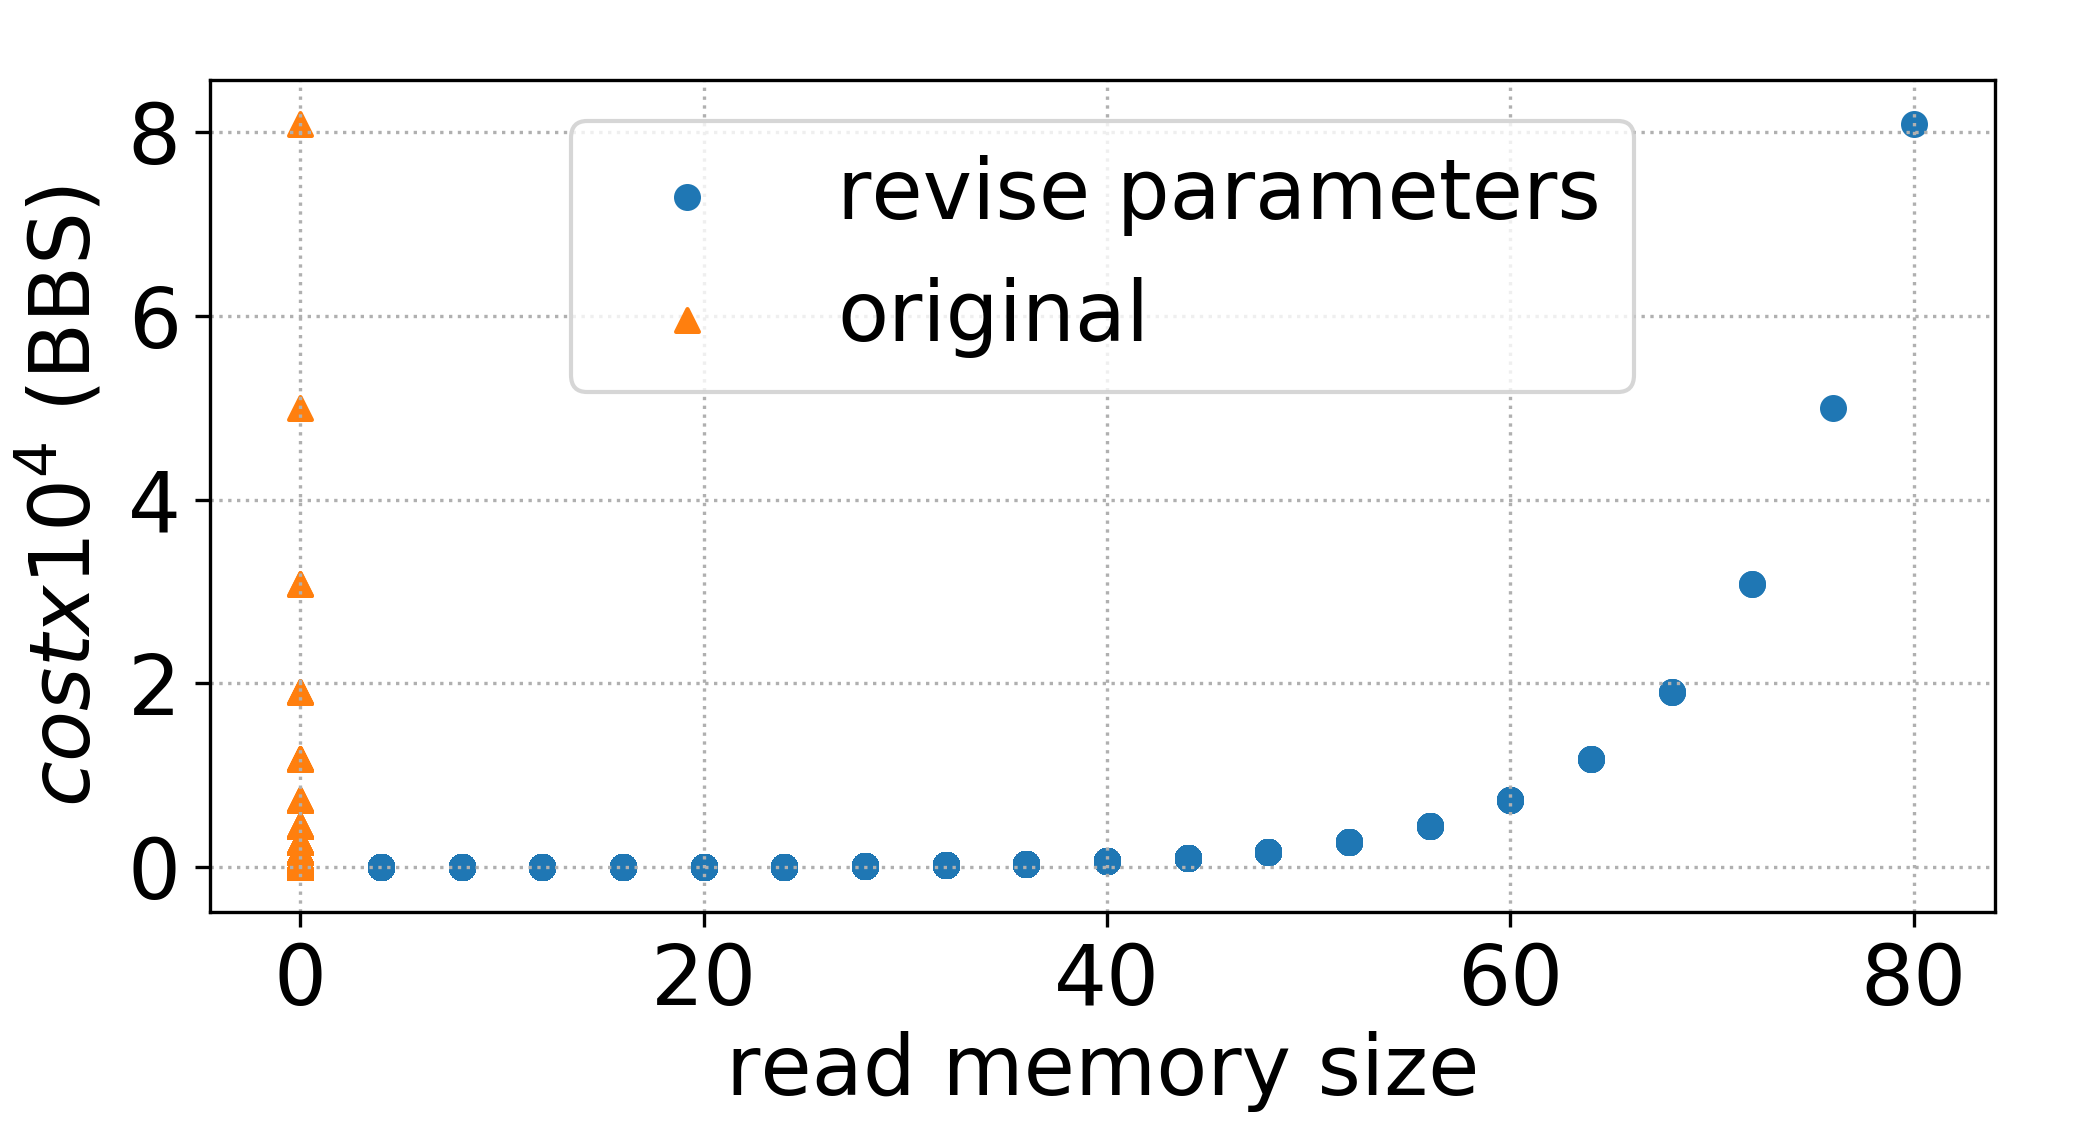
\includegraphics[width=0.24\linewidth]{figure/fib-line}\label{fig:fib-line}}
%\subfloat[Apache\#34464]{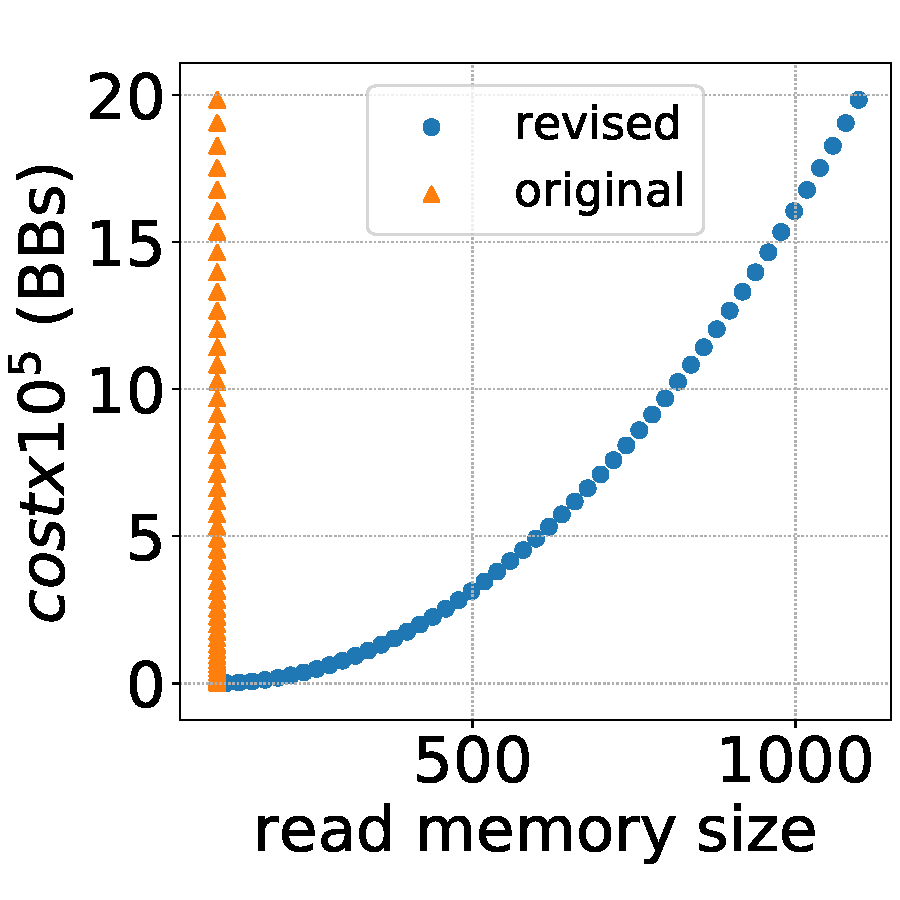
\includegraphics[width=0.24\linewidth]{figure/apache34464-line}\label{fig:apache34464-line}} \\ 
%\vspace{-0.1in}
%\caption{Cost function using RMS as input size. XXXXXX} 
%\label{fig:heat} 
%\end{figure*} 


%{{\bf{\underline{\textit{Input designs.}}}}
\subsubsection{How to design input metric?}
Many metrics can be used to measure input for a code construct. 
We discuss commonly used ones as follows.

\underline{\textit{Program input.}}
As discussed in Section~\ref{sec:process}, 
users tend to specify how to change the whole program 
input in order to describe the perceived complexity problem.
It is fairly easy to measure input size for the whole program based on users' report.
One way to measure input size for a code construct
is to simply use the input size of the whole program. 


\underline{\textit{Read memory size.}}
%Read memory size (RMS)is proposed as input size metric~\cite{Aprof1,Aprof2} . 
Read memory size (RMS) is defined as the number of distinct memory cells 
whose first access is read. 
RMS consider reads conducted by a code construct directly 
and reads conducted by 
functions called from the code construct. 


%\begin{figure}
%\centering
%\subfloat[Inner loop]{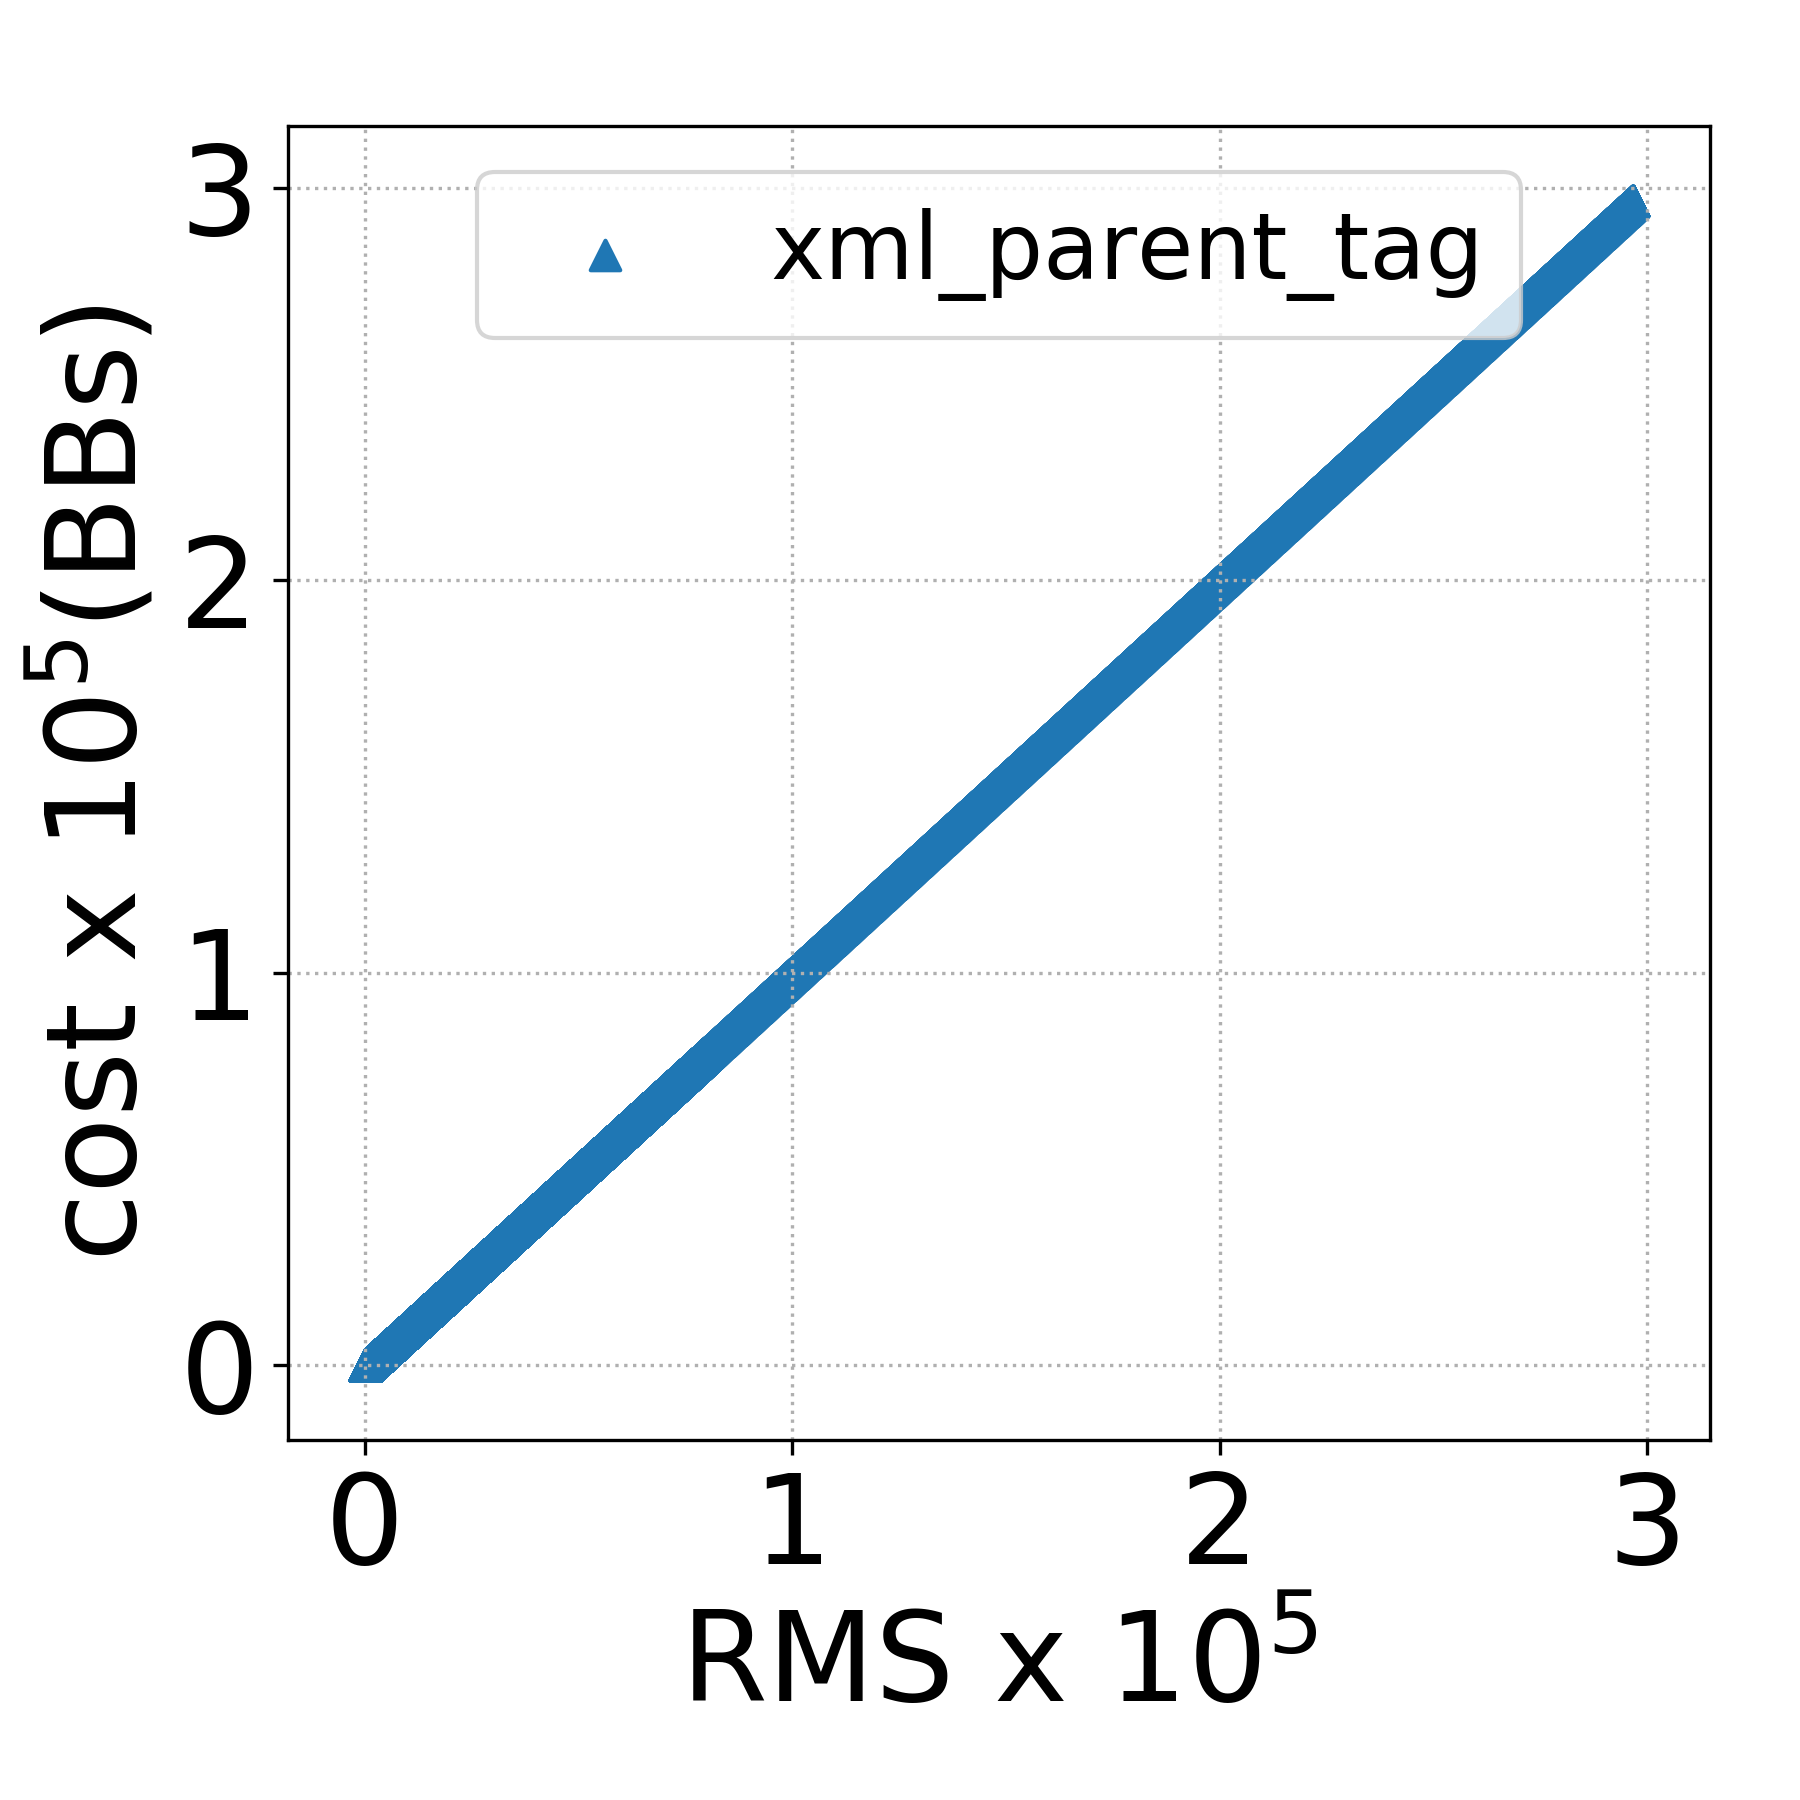
\includegraphics[width=0.42\linewidth]{figure/mysql27287-complexity-n}\label{fig:mysql27287-in}}
%\subfloat[Outer loop]{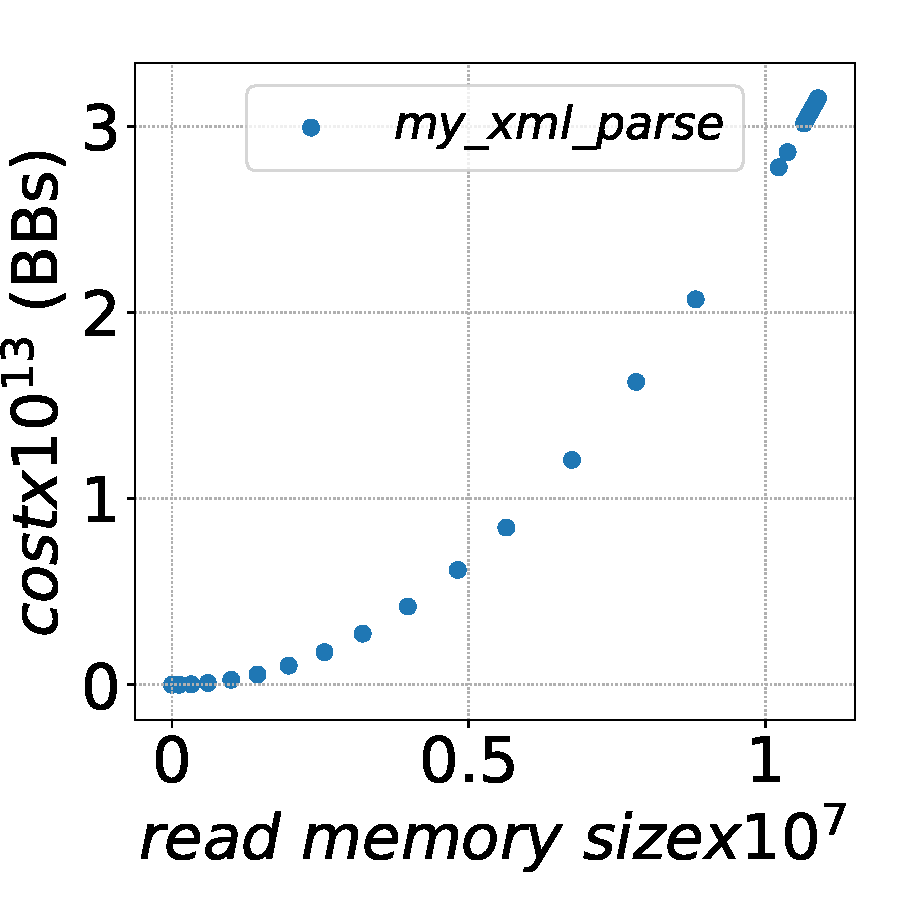
\includegraphics[width=0.42\linewidth]{figure/mysql27287-complexity-n-square}\label{fig:mysql27287-out}} \\ 
%\vspace{-0.1in}
%\caption{Inferred cost functions for MySQL\#27287 using RMS as input size.
%\footnotesize{(\texttt{xml\_parent\_tag} is the function containing the inner loop, 
%and \texttt{my\_xml\_parse} is the function containing the outer loop.)}} 
%\label{fig:mysql27287-2} 
%\end{figure} 

RMS is a generic metric for input size, 
and it can provide important input information for many complexity problems.   
For example, 
RMS for one execution of
the buggy loop in Figure~\ref{fig:mysql27287}
is roughly equal to 2 times the number of \texttt{XML\_NODE} 
accessed during the execution, 
because \texttt{level} field and \texttt{type} field of 
different \texttt{XML\_NODE}s are read in different loop iterations.
Although variable \texttt{p} and \texttt{level} are also read in each iteration,
RMS only considers distinct memory cells and 
only increases its value for the first read on these two variables in the first iteration. 
There is also an outer loop, 
and the outer loop invokes \texttt{xml\_parent\_tag} 
for every \texttt{XML\_NODE} contained
in the same array \texttt{items}. 
For that outer loop, its RMS is in linear relationship 
with the size of array \texttt{items}, 
since RMS only considers distinct memory cells 
and multiple reads conducted on the same memory 
cell of array \texttt{items} will not increase RMS. 
The inferred cost functions for the two functions 
containing the inner and the outer loop using RMS as input metric are shown 
in Figure~\ref{fig:mysql27287-2}.

{\underline{\textit{Data structure size.}}}
The number of accessed elements of a data 
structure could also be used to measure 
input size for a code construct~\cite{AlgoProf}. 
Commonly used data structures include linked lists and arrays.
Using data structure size can provide more semantic information for 
analyzed code constructs.
For example, if we focus on array \texttt{items}, 
the input size for both 
inner loop and outer loop of MySQL\#27287 is 
the number of accessed elements of array \texttt{items}.
Developers can clearly see that cost of each execution 
of the inner loop is in linear relationship with accessed elements, 
while the cost of the outer loop is in $O(N^2)$ relationship. 

In the reminder of this paper, we will focus on RMS as input metric. 
We skip the whole program input, 
because it is related to the input of a code construct in various ways.
Changing the whole program input may not change input sizes for 
all code constructs. 
Using the input size of the whole program as input metric for a code construct
may lead to incorrect profiling results. 
We also skip data structure size,
because it is not a generic metric. 
We need to design and implement extra static and dynamic techniques 
to identify data structures and figure out their sizes.


\subsubsection{How to design cost metric?}
There are also a lot of metrics which can be used to measure execution cost, 
such as the number of executed instructions, 
the time elapsed during execution,
the number of executed basic blocks (BBs), 
loop iteration, 
the number of recursive function call instances, and so on.

During our in-house technique design, 
we focus on the number of executed BBs. 
We do not use execution time, 
because when a code construct takes very little time,
using execution time may not provide an accurate measurement. 
We do not use the number of executed instructions, 
because this number is highly correlated with the number of BBs. 
Loop iteration and the number of recursive call instances could be used as estimates 
for the number of BBs. 
We do not use these two when designing in-house algorithmic profiling, 
but we will leverage them when building production-run techniques.  
 

\subsection{Implementation optimizations}

Aprof~\cite{Aprof1, Aprof2} is an algorithmic profiling tool built on Valgrind. 
Aprof uses RMS as input metric and executed BBs as cost metric.
Complexity information will be attributed to functions after profiling. 
We use LLVM framework to build an in-house algorithmic profiling tool.
Our tool building starts from the instrumentation algorithms used in aprof. 
We design a set of optimizations to reduce the runtime overhead, 
while providing accurate results.
In this section, we will first overview instrumentation algorithms in aprof firstly, 
and we will then discuss our designed optimizations. 

\subsubsection{Background}
To count executed BBs and RMS for each dynamic function call instance,
aprof runtime needs to maintain 5 global variables:
\texttt{cost}, 
tracking how many basic blocks are executed since the monitored program starts running, 
\texttt{count}, 
maintaining the current timestamp and increased by 1 after each function invocation, 
\texttt{ts}, 
a hash table containing the latest access timestamp for each memory cell,
\texttt{S}, 
a shadow stack tracking all active functions, 
and \texttt{top}, 
tracking the top of \texttt{S}.

Aprof instruments hook functions for 4 types of instructions: 
\texttt{call}, \texttt{return}, \texttt{read}, and \texttt{write}. 
When a function is invoked, 
\texttt{call} hook function will increment timestamp variable \texttt{count}
and grow the shadow stack \texttt{S} by incrementing \texttt{top}.
When a function returns,
\texttt{return} hook function will 
generate a log 
containing the returning function's RMS and executed BBs.
Since RMS also considers memory reads conducted by 
invoked callee functions, 
\texttt{return} hook function will add 
the RMS of the returning function to its caller on the stack. 
\texttt{read} hook function needs to query the hash table \texttt{ts} to decide  
whether to increment RMS for the function on top of the shadow stack \texttt{S}.
Both \texttt{read} and \texttt{write} 
hook function will update hash table \texttt{ts}
to maintain the latest access timestamp for an accessed memory cell. 


%{{{\bf{\underline{\textit{Aprof overview.}}}}
%\subsubsection{Background}
%Aprof uses the number of executed basic blocks as cost metric.
%To measure this number, aprof keeps a global counter \texttt{cost}, 
%which tracks how many basic blocks are executed since 
%starting the monitored program.
%To figure out whether a memory cell is accessed by the same function invocation before,
%aprof keeps another global counter \texttt{count}, 
%which tracks how many functions have been invoked.  
%Aprof maintains a shallow stack \texttt{S}, 
%which grows as the monitored program makes a function invocation, 
%and shrinks as the monitored program returns. 
%Aprof uses the third global variable \\texttt{top} to track the top of \texttt{S}.
%Aprof also maintains a hashmap \texttt{ts}, 
%which tracks latest access function for each distinct memory cell. 

%Aprof instruments 4 types of instructions: \texttt{call}, 
%\texttt{return}, \texttt{read}, and \texttt{write}. 
%When the monitored program makes a function call,
%aprof will increase \texttt{count} and \texttt{top} by 1.
%The new added stack entry will be initialized as follows, 
%\texttt{top.ts=count}, 
%\texttt{top.rms=0} and \texttt{top.cost=cost}.  
%Where the monitored program returns,
%aprof will create a log based on the content inside \texttt{S[top]}
%contribute the rms 
%of the returned function to its caller by doing \texttt{S[top-1].rms+=S[top].rms},
%and shrink the stack. 
%For a memory read on a cell \texttt{w},
%if \texttt{w}'s last access timestamp \texttt{ts[w]} is smaller 
%than the timestamp when the current function is invoked \texttt{S[top].ts},
%aprof will increase the RMS value for the current function.
%Since aprof will contribute an invoked function's rms to its caller, 
%aprof will also check active functions on the shadow stack and 
%decrease their RMS when necessary..   
%Aprof will set memory cell \texttt{w}'s latest access time 
%for all memory \texttt{read} and \texttt{write} on \texttt{w}.
%{\bf xxxx: these two parameters are very bad}
%{\bf remember to discuss how to change function to loop}

\subsubsection{Optimizations}
We design several optimizations to reduce the 
runtime overhead for our LLVM implementation from two aspects:
we try to reduce the number of instrumentation sites, 
and we try to accelerate hook functions. 

{\underline{\textit{Optimization 1}}
Our first optimization is designed to efficiently count the number of executed BBs.
Instead of incrementing a global counter by 1 inside every BB,
we apply an algorithm to decide where to update the BB counter and how to update the BB counter. 
The algorithm was originally designed to 
efficiently count edge events through selectively instrumenting counter 
on control flow graph~\cite{event-counting}. 
It has already been proved to be able to conduct path 
profiling efficiently~\cite{peter-ase,path-profiling}.

To apply the algorithm, we first instrument a local counter 
\texttt{local\_cost} at the beginning of each function
and initialize its value to be 0. 
We will add the value of \texttt{local\_cost} to the 
global counter \texttt{cost} before 
every function's return.
After that, we only need to consider where to update \texttt{local\_cost} 
within a single function.
We design and implement intra-procedural 
control flow analysis to achieve this.
Since the original algorithm is design to count events on edge,
we split each basic block into two and label event number to be 1 
for the edge connecting the two split basic blocks.  
We label event number to be 0 for all other edges. 
We calculate spanning tree for the new control flow graph. 
Edges not in the spanning tree are called chords.
We apply the depth-first search algorithm proposed in~\cite{event-counting} 
to calculate on which chords we should increase 
\texttt{local\_cost} and how much values 
we should add to \texttt{local\_cost}.


{\underline{\textit{Optimization 2}}
The second optimization tries to improve the performance of 
lookuping hash table \texttt{ts}, 
containing latest access timestamp for each memory cell.
For memory read, 
aprof needs to query \texttt{ts} and decide 
whether or not RMS should be incremented.
For memory read and write, 
aprof needs to update \texttt{ts} by using the current timestamp \texttt{count}
for accessed memory cells. 

Instead of using hash table, 
we use page table to contain timestamp information. 
To balance runtime overhead and memory overhead, 
we design a 4-layer page table for 32-bit programs.
We use 4 KB consecutive memory areas to hold pointers pointing to 
memory areas in the next layer 
or memory areas holding timestamps for memory cells. 
For a monitored 32-bit program, 
we need to calculate 4 addresses using bitwise operations 
and use the 4 addresses to refer each layer of the page table.  
For 64-bit programs, we use 6 layers.  


Compared with hash table, 
page page leverage locality of memory access 
and can lead 
to a better cache performance. 
To further improve performance, 
we add an extra variable to hold the pointer pointing 
to the last referred memory area holding timestamp.
For each memory read or write, 
we first check the saved pointer value can be used. 
We only conduct page table lookup, when the save value cannot be used. 

{\underline{\textit{Optimization 3}}
The third optimization targets reducing the number of instrumentation sites 
for \texttt{read} and \texttt{write}. 
We apply dominance analysis on 
control flow graph to achieve this.
For this optimization, we focus on stack memory cells holding 
scalar variables and only having \texttt{read} and \texttt{write} as uses 
(e.g. not having ``address of'' as uses).
We only focus on these memory cells,
because we want to avoid pointer alias analysis, 
which may potentially introduce inaccurate results. 
For a \texttt{read} instruction on one of these memory cells, 
if it is dominated by another \texttt{read} or \texttt{write} instruction 
on the same memory cell, we will skip to instrument this \texttt{read} instruction.
For a \texttt{write} instruction on one of these memory cells, 
if it is dominated by another \texttt{write} on the the same cell, 
we skip to instrument this \texttt{write}. 
{\bf xxx: add some numbers here}

 
{\underline{\textit{Optimization 4}}
For the last optimization, we apply inline functionality 
provide by LLVM to make all instrumented hook functions inline.


\subsection{Enhancing RMS}
There are two limitations in RMS. 
In this section, we will discuss how to augment  
RMS in order to address these two limitations.


\begin{figure}
\centering
\lstset{basicstyle=\ttfamily\fontsize{7}{8}\selectfont,
     morekeywords={+},keepspaces=true,numbers=left}
  \mbox{\lstinputlisting[mathescape,boxpos=t]{figure/fib.c}}
\caption{A recursive function to compute fibonacci number. 
(Execution time scales exponentially in the value of parameter \texttt{n}.) }
\vspace{-0.05in}
\label{fig:fib}
\vspace{-0.05in}
\end{figure}

\begin{figure}
\centering
\subfloat[fib]{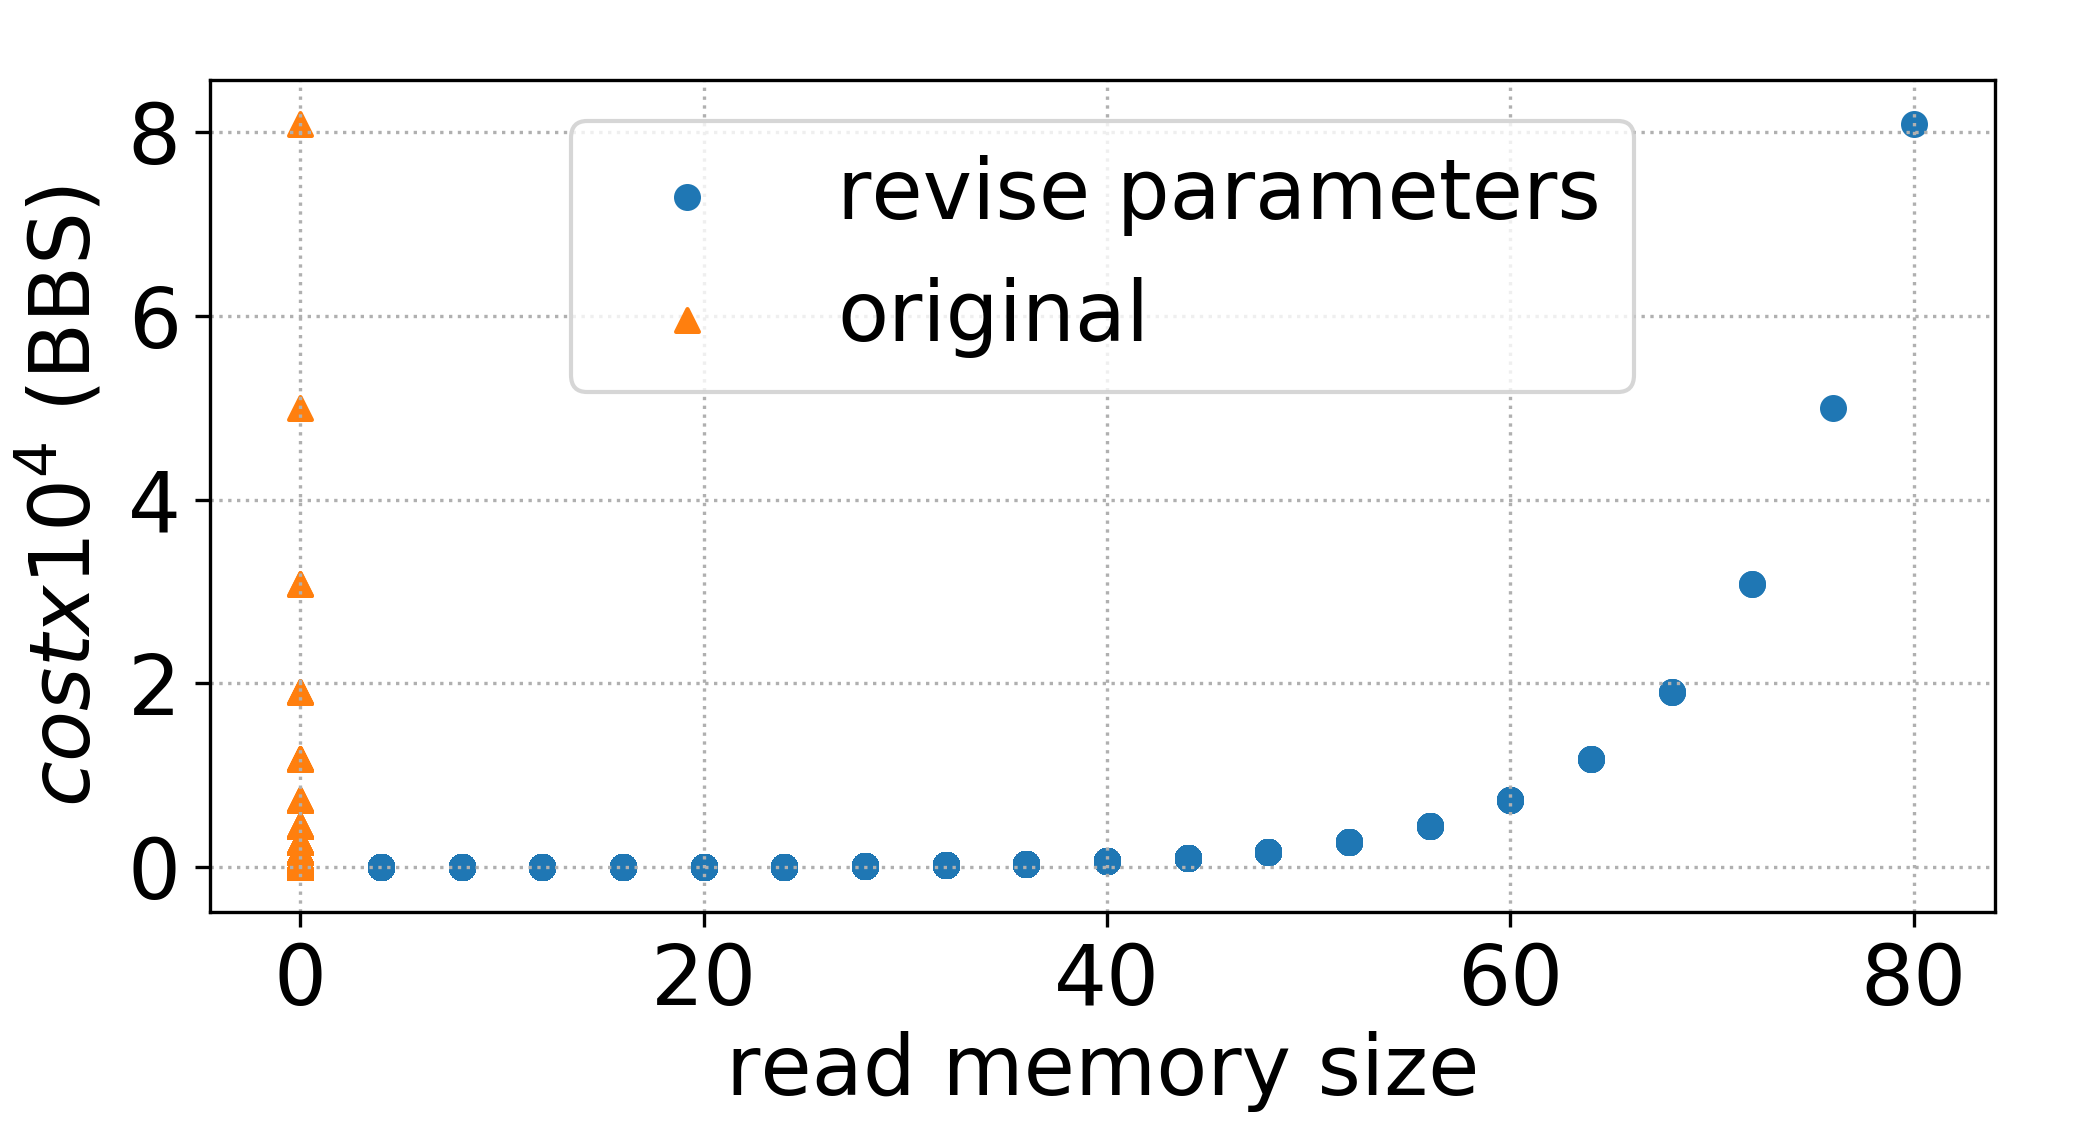
\includegraphics[width=0.42\linewidth]{figure/fib-line}\label{fig:fib-line}}
\subfloat[Apache\#34464]{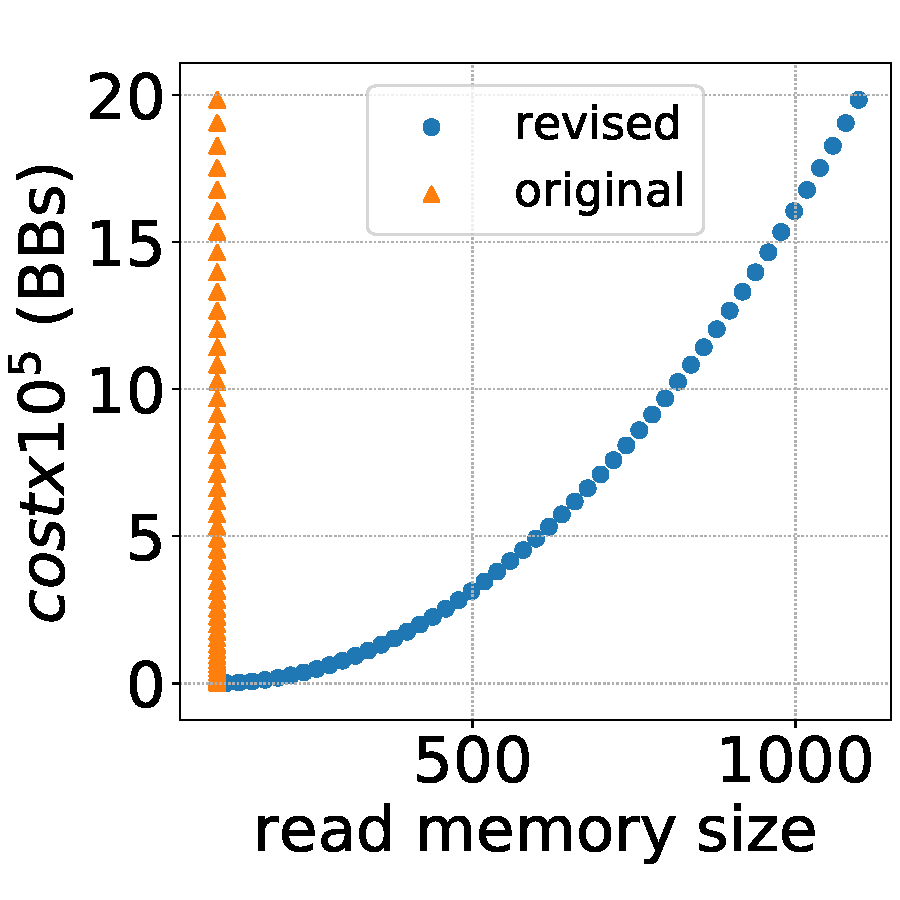
\includegraphics[width=0.42\linewidth]{figure/apache34464-line}\label{fig:apache34464-line}} \\ 
\vspace{-0.1in}
\caption{Cost function using RMS as input size. XXXXXX} 
\label{fig:heat} 
\end{figure} 

First, RMS cannot accurately measure input size for 
a recursive function
whose computation scales with the value of input parameter. 
Take the recursive function in Figure~\ref{fig:fib} as an example,
\texttt{fib} is to compute fibonacci number for parameter $n$.
For an invocation of \texttt{fib}, 
the first \texttt{read} on parameter $n$ will increment RMS.
However, after that, no matter how large $n$ is, RMS will not increment any more. 
This is because whenever \texttt{fib} recursively call itself on line 3, 
it needs to write parameter $n-1$ (or $n-2$) onto stack firstly, 
which means that the memory cell is accessed 
with \texttt{write} operation firstly.
To address this problem, when a function recursively call itself, 
we will increment RMS of the current function 
by the size of function call parameters. 
For example, when a call instance of $fib$ recursive calls itself 
($fib(n-1)$ or $fib(n-2)$) on line 3,
we will increment its RMS by 4.
The plots for $fib$ before and after algorithm 
adjustment is shown in Figure~\ref{fig:fib-line}.
Before adjustment, 
RMS will always be the same plotted 
as the vertical line on the left. 



\begin{figure}
\centering
\lstset{basicstyle=\ttfamily\fontsize{7}{8}\selectfont,
     morekeywords={+},keepspaces=true,numbers=left}
  \mbox{\lstinputlisting[mathescape,boxpos=t]{figure/apache34464.c}}
\caption{An Apache performance problem in $O(N^2)$ complexity. 
(Execution time scales polynomially in the number of characters read from  \texttt{getchar()}.) }
\vspace{-0.05in}
\label{fig:apache34464}
\vspace{-0.05in}
\end{figure}

Second, RMS does not consider inputs from I/O.
Buggy code fragment for Apache\#34463 is shown 
in Figure~\ref{fig:apache34464}.
The \texttt{while} loop on line 4 searches a string \texttt{source} for a target sub-string \texttt{target}.
If the \texttt{while} loop cannot find, 
a new character from I/O function \texttt{getchar()} 
on line 6 will be appended to string \texttt{source}, 
and the loop will search string \texttt{source} again from the beginning. 
The input size for this piece of codes depend on how many 
characters got from \texttt{getchar()}.
The computation scales polynomially as the input size.
Since all memory cells of string \texttt{source} are written 
firstly using return value of \texttt{getchar()}, 
no matter how many characters we get from \texttt{getchar()}, 
RMS of this piece of code only depends 
on the size of string \texttt{target}, 
variable \texttt{sourceLen} and variable \texttt{targetLen}.
To address this problem, 
we keep a list of I/O functions. 
When these functions are called, 
we will increment RMS for all 
functions active on the shadow stack. 
The plots for the function containing the buggy loop 
before and after algorithm adjustment is shown in Figure~\ref{fig:apache34464-line}.
Before adjustment, 
RMS will always be the same no 
matter how many characters received from \texttt{getchar()}. 


\subsection{Discussions}

RMS considers memory reads conducted by functions called from a code construct,
while it does not consider memory accesses 
by the same code construct from different executions.
Basically, RMS measures input size in a top-down view.
In the next section, we will discuss why it is difficult to apply sampling to RMS.

All the optimizations proposed in this section can reduce runtime overhead 
without changing profiling results.
Approximate algorithms could be explored to further reduce overhead. 
For example, in our current implementation, 
we use byte as unit for distinct memory cells.
We could explore to use larger units, like 4 bytes or 16 bytes. 
Using a larger unit can reduce both memory overhead and runtime overhead for the page table,
but the timestamp information contained is not precise.  
As another example, we could leverage alias analysis 
and extend our dominance analysis other \texttt{read} and 
\texttt{write} operations.  
We will leave the exploration of approximate algorithms for future works.  
 
There are many new hardware with the potential to replace 
software instrumentation discussed in this section and further reduce runtime overhead. 
For example, Intel Processor Tracer (PT) could be used to count executed BBs. 
We will also leave the exploration of new hardware for future works.  

\begin{table}[h!]
  \centering
  \scriptsize
  \newcommand{\Yes}[1]{\checkmark{}$_#1$}
  \newcommand{\No}[0]{-}
  \begin{tabular}{lccccccccccc}
    \toprule     
    {\bf BugID}                   & KLOC  &  P.L.    & \multicolumn{6}{c}{\# of Static Features}                      &   Complexity  & Buggy C.C.        & \# of Inputs \\
                           
    \cmidrule(lr){4-9}
                                  &       &          &  BB      &  Loop     & A-L    &  LL-L    &  Function  & R.F.          &           &        &  \\
    \midrule 

    Mozilla\#347306              &  $88$    & C        &   46735  &   1177     &  483    &  136    &  1988  & 35   &  $O(N^{2})$                         &  A-L  & 10000   \\
    Mozilla\#416628              &  $105$   & C        &   46097  &   1116     &  484    &  136    &  1919  &  35  &  $O(N^{2})$                         &  LL-L & 380  \\
    Mozilla\#490742              &  $0.157^*$    & JS         &  41     & 4       &  3     &   0  &  8           &  0   & $O(N)$        &  A-L  &  10000              \\
    Mozilla\#35294               &  $0.195^*$  & C++  & 85 &  9  &  5  & 0  & 12   & 0                                  &  $O(N^{2})$   &  Loop & 50000  \\
    Mozilla\#477564              &  $0.116^*$  & JS  & 40 & 6 & 1 & 3 & 5   & 0                                         & $O(N^{2})$    &  LL-L & 4000       \\
    \midrule
    MySQL\#27287                 &  $995$  & C++  & 88971  & 2535 & 905 & 287 & 11969 & 80                                                          & $O(N^{2})$    & A-L   & 65536            \\
    MySQL\#15811      &  $1127$ & C++  & 17656 & 844 & 237 & 29 & 490 & 5                                                                &  $O(N^{2})$   & A-L   & 16384 \\
    \midrule
    Apache\#37184     &  $0.092^*$ & Java  & 31 & 5  & 0 & 0 & 7 & 0                                                    & $O(N)$        & Loop & 10000     \\ 
    Apache\#29743     &  $0.257^*$  & Java  & 408 & 8 & 0 & 0 & 123 & 0                                                 & $O(N^{2})$    & Loop & 10000 \\
    Apache\#34464     &  $0.16^*$  & Java  & 70 & 6 & 5 & 0  & 13 & 0                                                   & $O(N^{2})$    & A-L  & 50000 \\
    Apache\#47223     &  $0.162^*$ & Java  & 67 & 5 & 4 & 0  & 13 & 0                                                   & $O(N^{2})$    & A-L  & 50000 \\
    \midrule
    GCC\#46401        &  $5521$  & C  & 301913 & 11266 & 1340 & 1637 & 27733 & 964                                                       & $O(N^{2})$    & LL-L & 1462 \\
    GCC\#1687         &  $2099$  & C  & 125408 & 5315  & 724 & 1086  & 7573  & 558                                                       & $O(2^{N})$    & R.F. & 16  \\
    GCC\#27733        &  $3217$  & C  & 217239 & 7412 & 1004 & 1196  & 12722 & 686                                                       & $O(2^{N})$    & R.F. & 65  \\
    GCC\#8805         &  $2538$  & C  & 148099 & 5857 & 841 & 1222 & 6753 & 517                                                          & $O(N^{2})$    & LL-L & 1000 \\
    GCC\#21430        &  $3844$  & C  & 283675 & 7727 & 883  & 1178 & 13745 & 700                                                        & $O(N^{2})$    & LL-L & 10000 \\
    GCC\#12322        &  $2341$  & C  & 124310 & 5397 & 831 & 1190 & 7078 & 540                                                          & $O(N^{2})$    & LL-L & 1175 \\
    \midrule
    \midrule
    Apache\#53622     & $1.094^*$  & Java  & 345 & 38 & 22 & 12 & 72 & 0                                                & $O(N^{2})$    & A-L & 50000    \\
    Apache\#53637     & $0.937^*$  & Java  & 308 & 34 & 21 & 9  & 60 & 0                                                & $O(N^{2})$    & A-L & 50000 \\
    Apache\#53803     & $0.421^*$  & Java  & 128 & 11 & 9  & 0  & 34 & 0                                                & $O(N^{2})$    & A-L & 50000     \\
    Apache\#53821     & $0.417^*$  & Java  & 131 & 12 & 10 & 0  & 34 & 0                                                & $O(N^{2})$    & A-L & 50000      \\
    Apache\#53822     & $0.417^*$  & Java  & 132 & 12 & 11 & 0  & 34 & 0                                                & $O(N^{2})$    & A-L & 50000      \\
    \midrule
    Collections\#406      & $0.253^*$  & Java  & 81 & 9 & 7 & 0 & 19 & 0                                                  & $O(N^{2})$ & A-L & 50000      \\
    Collections\#407      & $0.766^*$  & Java  & 234 & 26 & 15 & 9 & 53 & 0                                               & $O(N^{2})$ & A-L & 50000   \\
    Collections\#408      & $0.742^*$  & Java  & 225 & 25 & 14 & 9 & 51 & 0                                               & $O(N^{2})$ & A-L & 50000    \\
    Collections\#409      & $0.781^*$  & Java  & 236 & 26 & 15 & 9 & 53 & 0                                               & $O(N^{2})$ & A-L & 50000     \\
    Collections\#410      & $0.769^*$ & Java   & 234 & 26 & 15 & 9 & 51 & 0                                               & $O(N^{2})$ & A-L & 50000    \\
    Collections\#412      & $0.284^*$  & Java  & 84 & 9  & 6  & 0  & 20 & 0                                               & $O(N^{2})$ & A-L & 50000     \\
    Collections\#413      & $0.923^*$  & Java  & 274 & 32 & 16 & 14 & 62 & 0                                              & $O(N^{2})$ & LL-L & 50000   \\
    Collections\#425      & $0.758^*$  & Java  & 233 & 26 & 15 & 9  & 52 & 0                                              & $O(N^{2})$ & A-L & 50000    \\
    Collections\#426      & $0.783^*$  & Java  & 242 & 26 & 15 & 9  & 53 & 0                                              & $O(N^{2})$ & A-L & 50000   \\
    Collections\#427      & $0.756^*$ & Java  & 227 & 25 & 14 & 9  & 53 & 0                                               & $O(N^{2})$ & A-L & 50000   \\
    Collections\#429-0    & $0.668^*$  & Java  & 203 & 21 & 11 & 7 & 45 & 0                                             & $O(N^{2})$ & Loop & 30000       \\
    Collections\#429-1    & $0.536^*$  & Java  & 157 & 20 & 13 & 4 & 36 & 0                                             & $O(N^{2})$ & Loop & 30000     \\
    Collections\#429-2    & $0.416^*$ & Java  & 129 & 15 & 9 & 3  & 26 & 0                                             & $O(N^{2})$ & Loop & 30000 \\
    Collections\#434      & $0.336^*$  & Java  & 86  & 10 & 0 & 8 & 33 & 0                                               & $O(N^{2})$ & LL-L & 50000     \\
    \midrule
    Groovy\#5739-0        & $0.745^*$  & Java  & 227 & 10 & 0 & 8 & 51 & 0                                                & $O(N^{2})$ & LL-L& 50000 \\
    Groovy\#5739-1        & $0.756^*$  & Java  &227  & 25 &  14 & 9 & 51 & 0                                              & $O(N^{2})$ & A-L & 50000 \\
    \midrule
    \midrule
    knapsack      &  $0.282$  & C++  & 42 & 1 & 0 & 0 & 5 & 1                                                                            & $O(2^{N})$ & R.F. & 30  \\
    fib      &  $0.048$ & C++  & 10 & 0 & 0 & 0 & 3 & 1                                                                                  & $O(2^{N})$ & R.F. & 45 \\
    parentheses      & $0.056$   & C++  & 10 & 0 & 0 & 0 & 3 & 1                                                                         & $O(2^{N})$ & R.F. & 19 \\
    nqueens      & $0.091$  & C++  & 33 & 3 & 2 & 0 & 4 & 1                                                                              & $O(2^{N})$ & R.F. & 13 \\
    graphcol      &  $0.171$  & C++  & 58 & 8 & 3 & 0 & 8 & 1                                                                            & $O(2^{N})$ & R.F. & 50 \\
    uts      &  $0.667$  & C++  & 40  & 2 & 0 & 0 & 8 & 1                                                                                & $O(N)$     & R.F. & 20 \\
    binomial      &  $0.058$  & C++  & 14 & 0 & 0 & 0 & 3 & 1                                                                            & $O(2^{N})$ & R.F. & 36 \\
    minmax      &  $0.262$  & C++  & 203 & 8 & 3 & 0 & 8 & 1                                                                             & $O(2^{N})$ & R.F. & 13 \\


    \bottomrule
   \end{tabular}
  %\nocaptionrule
  \caption{Benchmark Information.
  \footnotesize{(This table shows information for complexity problems used in our evaluation. 
   $x^*$: thousands of lines of codes for re-implemented benchmarks; 
   A-L: array-processing loop; 
   LL-L: linked-list-processing loop; 
   R.F.: recursive function; 
   Buggy C.C.: buggy code construct.)}}
  \label{tab:benchmark_info}
\end{table}
\begin{table*}[h!]
  \centering
  \scriptsize
  \newcommand{\Yes}[1]{\checkmark{}$_#1$}
  \newcommand{\No}[0]{-}
  \begin{tabular}{lccccccccccc}
    \toprule
    {\bf BugID}                   & KLOC  &  P.L.    & \multicolumn{6}{c}{\# of Static Features}                                          &   Complexity  & Buggy C.C.        & \# of Inputs \\

    \cmidrule(lr){4-9}
                                 &        &          &  BB      &  Loop     & A-L    &  LL-L    &  F.  & R.F.                             &               &                             & \\
    \midrule

    Mozilla\#347306              &  88    & C        &          &           &       &           &       &                                 &               &&         \\
    Mozilla\#416628              &  105   & C        &          &           &       &           &       &                                 &               &&                \\
    Mozilla\#490742                  &  -  & JS  &  &              &    &                                 &                   &                           &       &&                         \\
    Mozilla\#35294    &  -  & C++  &  &              &    &                                 &                   &                           &                     &&          \\
    Mozilla\#477564   &  -  & JS  &  &              &    &                                 &                   &                           &                      &&          \\
    \midrule
    MySQL\#27287      &  995  & C++  &  &              &    &                                 &                   &                           &                   &&             \\
    MySQL\#15811      &  1127 & C++  &  &              &    &                                 &                   &                           &                   &&             \\
    \midrule
    Apache\#37184     &  -  & Java  &  &              &    &                                 &                   &                           &                    &&           \\
    Apache\#29743     &  -  & Java  &  &              &    &                                 &                   &                           &                    &&          \\
    Apache\#34464     &  -  & Java  &  &              &    &                                 &                   &                           &                    &&           \\
    Apache\#47223     &  -  & Java  &  &              &    &                                 &                   &                           &                    &&           \\
    \midrule
    GCC\#46401        &  5521  & C  &  &              &    &                                 &                   &                           &                    &&            \\
    GCC\#1687         &  2099  & C  &  &              &    &                                 &                   &                           &                    &&           \\
    GCC\#27733        &  3217  & C  &  &              &    &                                 &                   &                           &                    &&           \\
    GCC\#8805         &  2538  & C  &  &              &    &                                 &                   &                           &                    &&            \\
    GCC\#21430        &  3844  & C  &  &              &    &                                 &                   &                           &                    &&            \\
    GCC\#12322        &  2341  & C  &  &              &    &                                 &                   &                           &                    &&           \\
    \midrule
    \midrule
    Apache\#53622     &  -  & Java  &  &              &    &                                 &                   &                           &                    &&           \\
    Apache\#53637     &  -  & Java  &  &              &    &                                 &                   &                           &                    &&          \\
    Apache\#53803     &  -  & Java  &  &              &    &                                 &                   &                           &                    &&            \\
    Apache\#53821     &  -  & Java  &  &              &    &                                 &                   &                           &                    &&           \\
    Apache\#53822     &  -  & Java  &  &              &    &                                 &                   &                           &                    &&            \\
    \midrule
    Collections406    &  -  & Java  &  &              &    &                                 &                   &                           &                    &&           \\
    Collections407    &  -  & Java  &  &              &    &                                 &                   &                           &                    &&          \\
    Collections408    &  -  & Java  &  &              &    &                                 &                   &                           &                    &&            \\
    Collections409    &  -  & Java  &  &              &    &                                 &                   &                           &                    &&            \\
    Collections410    &  - & Java  &  &              &    &                                 &                   &                           &                     &&           \\
    Collections412    &  -  & Java  &  &              &    &                                 &                   &                           &                    &&            \\
    Collections413    &  -  & Java  &  &              &    &                                 &                   &                           &                    &&            \\
    Collections425    &  -  & Java  &  &              &    &                                 &                   &                           &                    &&            \\
    Collections426    &  -  & Java  &  &              &    &                                 &                   &                           &                    &&            \\
    Collections427    &   - & Java  &  &              &    &                                 &                   &                           &                    &&            \\
    Collections429-0    &  -  & Java  &  &              &    &                                 &                   &                           &                  &&              \\
    Collections429-1    &  -  & Java  &  &              &    &                                 &                   &                           &                  &&              \\
    Collections429-2    &  -  & Java  &  &              &    &                                 &                   &                           &                  &&              \\
    Collections434    & -   & Java  &  &              &    &                                 &                   &                           &                    &&            \\
    \midrule
    Groovy5739-0      & -  & Java  &  &              &    &                                 &                   &                           &                     &&           \\
    Groovy5739-1      & -  & Java  &  &              &    &                                 &                   &                           &                     &&          \\
    \midrule
    \midrule
    knapsack      &  -  & C++  &  &              &    &                                 &                   &                           &                         &&     \\
    fib      &  - & C++  &  &              &    &                                 &                   &                           &                               && \\
    parentheses      & -   & C++  &  &              &    &                                 &                   &                           &                      &&          \\
    nqueens      &  -  & C++  &  &              &    &                                 &                   &                           &                          &&      \\
    graphcol      &  -  & C++  &  &              &    &                                 &                   &                           &                         &&     \\
    uts      &  -  & C++  &  &              &    &                                 &                   &                           &                              && \\
    binomial      &  -  & C++  &  &              &    &                                 &                   &                           &                         &&       \\
    minmax      &  -  & C++  &  &              &    &                                 &                   &                           &                           &&    \\


    \bottomrule
   \end{tabular}
  %\nocaptionrule
  \caption{Run-time overhead and diagnosis capability evaluated with the default sampling rate (1 out of 10000); 10, 100, 500, 1000 represents the different numbers of success/failure runs used for diagnosis.}
  \label{tab:LBR}
\end{table*}

%\newpage
\section{Production-Run Algorithmic Profiling}
\label{sec:online}

In this section, we discuss our design and 
implementation for the production-run version of \Tool. 
For production-run usage, profiles are collected from the user side.
It is very important to keep the runtime overhead low, since
end users cannot tolerate any observable performance slowdown.
To achieve this requirement,
our design follows several principles. 

First, \textit{study guided}. 
The design of the production-run version of \Tool
is guided by the empirical study in Section~\ref{sec:study}.
We focus on the majority of complexity problems, 
caused either by repeated executions of a loop ($N^k$)
or a recursive function ($2^N$).
We focus on common types of data structures, which are array and linked list.

Second, \textit{focused checking}.
When applying the production-run version of \Tool, 
we expect developers will specify a suspicious loop or a suspicious recursive function
to be monitored. 
\Tool will automatically instrument the specified code construct 
to collect runtime information from the user side in a low overhead. 
The profiling results can help developers better understand the complexity of the code construct 
and its processed workloads in the real world.
\Tool can be used together with performance failure 
diagnosis tools~\cite{SongOOPSLA2014} 
or traditional profilers to
focus on suspicious code constructs leading 
to user-perceived performance failures.

Third, \textit{sampling}.
Instead of recording all dynamic information, 
we apply sampling and record only part of the information. 
We infer information for the whole execution based on the collected samples. 
Sampling can effectively lower the runtime overhead. 


\subsection{Technical Design}
As we discussed in Section~\ref{sec:study}, 
the majority of complexity problems studied are caused 
by repeated executions of a loop or a recursive function. 
Previous works show that sampling code constructs that are executed 
multiple times in one program run can lower the runtime overhead, 
while still being able to collect enough runtime information 
without hurting diagnosis latency~\cite{SongOOPSLA2014,ldoctor}. 
Inspired by our study and the earlier works, 
we apply sampling to efficiently profile loops 
and recursive functions with multiple executions. 

\noindent\textbf{Input Metric}
If the specified code construct is an array-processing loop 
or a linked-list-processing loop,
we will use DSS as the input metric. 
Otherwise, we will use RMS+ as the input metric. 

As we discussed in Section~\ref{sec:inhouse}, 
there are two methods, top-down and bottom-up, 
to analyze RMS+ and DSS records collected 
for multiple dynamic instances of a code construct in one program run. 
We leverage the top-down method for the in-house version of \Tool. 
However, the top-down method is not suitable for sampling. 
The reason is as follows.
Assume we have a code construct \texttt{c} to monitor. 
It is inside a loop \texttt{l} and is executed multiple times in one program run.
There are fewer dynamic instances of \texttt{l}
than dynamic instances of \texttt{c}.
If we apply the top-down method, 
we need to sample dynamic instances of \texttt{l}, 
and it is very likely that we will miss these instances. 
For each dynamic instance of \texttt{l}, 
there will be more computation, 
compared with an instance of \texttt{c}.
More overhead will be incurred to collect 
information for dynamic instances of \texttt{l}.
Therefore, we apply the bottom-up method 
in the production-run version of \Tool.
We sample instances of \texttt{c} to record 
distinct memory cells contributing RMS+ 
or distinct elements in an array or a linked list.
We use the sampled information to infer RMS+ 
or DSS for all instances of \texttt{c} in one program run.


The sampling method is similar to that described in previous works on statistical 
debugging~\cite{liblit03,liblit05,CCI,SongOOPSLA2014,ldoctor}.
We make a cloned version of the monitored code construct.
We instrument the cloned version to record information for RMS+ or DSS. 
We dump the recorded information to log 
whenever the cloned version finishes execution. 
We add extra delimiters to log to differentiate information collected from different instances.
Before each execution of the monitored code construct, 
we choose between the cloned version and the original version. 
How many times the cloned version is executed 
depends on a tunable sampling rate. 
To make the choice between the two versions,
we add a global counter to the monitored program. 
If the counter value is larger than $0$, 
we choose the original version and decrease the counter value by $1$.
If the counter value is equal to $0$,
we choose the cloned version and reset the counter value to 
a random number, 
whose expectation is equal to the inverse of the sampling rate.  


We leverage the mark-and-recapture method~\citep{mark-recapture} to 
estimate RMS+ or DSS for all dynamic instances of a code construct 
based on the collected samples. 
Mark-and-recapture is a commonly used statistical method 
for estimating the size of an animal population. 
In this method, some of the animals are captured, marked, and released. 
Then, another group of the animials are captured.
The size of the whole animal population is estimated 
based on the ratio of marked animals in the second captured sample.  


Each sample of a monitored code construct is a set of memory cells, 
which contribute RMS+ or represent distinct elements in an array or a linked list. 
In one program run, we assume that we collect a sequence of $m$ samples. 
Given the $i$th sample, $M_i$ represents the 
total number of distinct memory cells in the previous $i-1$ samples, 
$C_i$ represents the number of distinct memory cells in the $i$th sample,
and $R_i$ represents the number of distinct memory cells in 
the $i$th sample that also appeared in one of the previous $i-1$ samples.
The total number of distinct memory cells for all dynamic instances 
of the monitored code construct can be estimated as:


%\begin{equation} \label{eq:mark}
%$$p_v(S_v(a)) = 1 - \prod\limits_{u \in S_v(a)}(1 - p_{u,v})$$
%N = \frac{\sum\limits_{i=1}^m M_i*C_i}{\sum\limits_{i=1}^m R_i}
%\end{equation}

\begin{equation} \label{eq:mark}
N = \sum\limits_{i=1}^m M_i*C_i\Big/\sum\limits_{i=1}^m R_i
\end{equation}

\noindent\textbf{Cost Metric}
The production-run version of \Tool focuses on recursive functions or loops.
If the monitored code construct is a recursive function,
we use RIs as the cost metric.
If the monitored code construct is a loop, 
we use LIs as the cost metric. 
We do not apply sampling when collecting these two metrics. 
As we discussed in Section~\ref{sec:inhouse},
these two metrics will incur a smaller overhead compared with BBs, 
and they can still provide accurate profiling results.  


\subsection{Experimental Evaluation}
%\subsubsection{Research Questions}

\subsubsection{Methodology}
We will conduct experiments to answer the following two research questions:

\begin{itemize}
\item {\bf RQ1.} 
Can sampling lower the runtime overhead while giving the same profiling results? 
A positive answer means the effectiveness of the production-run version of \Tool. 

\item {\bf RQ2.} 
Will sampling increase the profiling latency? 
By applying sampling, less information is collected in one single run. 
If we have to monitor more program runs to get the same profiling results,
the profiling latency is increased.
As we discussed earlier, the majority of complexity problems are caused 
by repeated executions of a loop or a recursive function.
It is possible that sampling can still collect enough information in one program run, 
while not increasing the profiling latency. 


\end{itemize}

\noindent\textbf{Benchmarks and Inputs}
We reuse all benchmarks in Table~\ref{tab:benchmark_info}.
We monitor the loop or the recursive function with the most iterations\footnote{We consider a recursive function call instance as a loop iteration.} 
for all benchmarks,
except for Mozilla\#347306 and GCC\#46401. 
%These two bugs are caused repeated execution of a loop, 
%whose total iteration numbers ranked 2nd. 
%Instead, we monitor these two loops.
These two bugs are caused by the repeated executions of a loop with the second
highest number of iterations. Instead of using the loop with the most iterations,
we monitor these two loops.


For each benchmark, 
we use the same methodology described in Section~\ref{sec:inhouse_exp} 
to generate a sequence of inputs, 
so that the difference between the sizes of two consecutive inputs is constant.
This input set contains controlled inputs.
We also randomly sample controlled inputs to generate a set of random 
inputs to emulate the uncontrolled inputs in production runs.    

\noindent\textbf{Metrics}
We will measure the following three metrics during our experiments:
1) runtime overhead, which is the slowdown caused 
by sampling information from each program run;
2) profiling capability, which is measured as the similarity between two cost functions 
inferred under the in-house setting and the production-run setting using the same metrics;
and 3) profiling latency, which is measured by how many program 
runs are needed for the algorithmic profiling. 


\begin{table*}[h!]
\vspace{-0.05in}
  \centering
  \scriptsize
  \newcommand{\Yes}[1]{\checkmark{}$_#1$}
  \newcommand{\No}[0]{-}
  \begin{tabular}{lccccccccc}
    \toprule
   {\bf BugID}                   &  \multicolumn{4}{c}{Controlled Inputs}            &     \multicolumn{4}{c}{Random Inputs}          & Overhead \\

    \cmidrule(lr){2-5}
    \cmidrule(lr){6-9}
    (\# of runs)                 &  (10)     &   (100)    &    (500)    & (1000)     &  (10)     &   (100)    &    (500)    & (1000)   &   per run\\
    \midrule

    Mozilla\#347306   & \ding{51}$_{0.96}$ & \ding{51}$_{0.96}$  & \ding{51}$_{0.96}$ & \ding{51}$_{0.96}$ & \ding{51}$_{0.95}$ & \ding{51}$_{0.96}$ & \ding{51}$_{0.96}$ & \ding{51}$_{0.95}$ &  1.31\% \\
    Mozilla\#416628   & \ding{51}$_{0.94}$ & \ding{51}$_{0.95}$  & \ding{51}$_{0.96}$  & \ding{51}$_{0.96}$ & \ding{51}$_{0.88}$ & \ding{51}$_{0.94}$ & \ding{51}$_{0.95}$ & \ding{51}$_{0.95}$ & 0.32\% \\
    Mozilla\#490742   &  -  & -  & - & - & - & - & - & - & 0.33\% \\
    Mozilla\#35294    &  \ding{51}$_{0.99}$  & \ding{51}$_{0.97}$ & \ding{51}$_{0.98}$ & \ding{51}$_{0.98}$ & \ding{51}$_{0.97}$ & \ding{51}$_{0.97}$ & \ding{51}$_{0.98}$ & \ding{51}$_{0.98}$ & 0.94\% \\
    Mozilla\#477564   &  \ding{51}$_{0.98}$  & \ding{51}$_{0.99}$ & \ding{51}$_{0.99}$ & \ding{51}$_{0.99}$ & \ding{51}$_{0.93}$ & \ding{51}$_{0.96}$ & \ding{51}$_{0.97}$ & \ding{51}$_{0.97}$ & 4.55\% \\
    \midrule
    MySQL\#27287      &  \ding{51}$_{0.93}$  & \ding{51}$_{0.93}$ & \ding{51}$_{0.94}$ & \ding{51}$_{0.94}$ & \ding{51}$_{0.86}$ & \ding{51}$_{0.92}$ & \ding{51}$_{0.94}$ & \ding{51}$_{0.94}$& 2.92\% \\
    MySQL\#15811      &  \ding{51}$_{0.93}$  & \ding{51}$_{0.95}$ & \ding{51}$_{0.95}$ & \ding{51}$_{0.96}$ & \ding{51}$_{0.93}$ & \ding{51}$_{0.93}$ & \ding{51}$_{0.94}$ & \ding{51}$_{0.94}$ & 4.09\% \\
    \midrule
    Apache\#37184     &  -  & -  & - & - & - & - & - & - & 4.5\% \\
    Apache\#29743     & \ding{51}$_{0.85}$  & \ding{51}$_{0.85}$ & \ding{51}$_{0.86}$ & \ding{51}$_{0.86}$ & - & - & \ding{51}$_{0.85}$ & \ding{51}$_{0.85}$ & 0.61\% \\
    Apache\#34464     & \ding{51}$_{0.98}$  & \ding{51}$_{0.99}$ & \ding{51}$_{0.99}$ & \ding{51}$_{0.99}$ & \ding{51}$_{0.97}$ & \ding{51}$_{0.99}$ & \ding{51}$_{0.99}$ & \ding{51}$_{0.99}$ & 4.55\% \\
    Apache\#47223     & -  & \ding{51}$_{0.99}$ & \ding{51}$_{0.99}$ & \ding{51}$_{0.99}$ &\ding{51}$_{0.87}$ & \ding{51}$_{0.93}$ & \ding{51}$_{0.94}$ & \ding{51}$_{0.95}$ & 3.7\% \\
    \midrule
    GCC\#46401       & \ding{51}$_{0.89}$  & \ding{51}$_{0.91}$ & \ding{51}$_{0.91}$ & \ding{51}$_{0.92}$ & \ding{51}$_{0.86}$ & \ding{51}$_{0.88}$ & \ding{51}$_{0.91}$ & \ding{51}$_{0.91}$ & 3.5\% \\
    GCC\#1687        & \ding{51}$_{0.85}$  & \ding{51}$_{0.87}$ & \ding{51}$_{0.87}$ & \ding{51}$_{0.87}$ & - & \ding{51}$_{0.86}$ & \ding{51}$_{0.87}$ & \ding{51}$_{0.87}$ & 9.46\% \\
    GCC\#27733       & -  & \ding{51}$_{0.85}$ & \ding{51}$_{0.85}$ & \ding{51}$_{0.85}$ & - & \ding{51}$_{0.86}$ & \ding{51}$_{0.86}$ & \ding{51}$_{0.86}$ & 0.92\% \\
    GCC\#8805        & -  & \ding{51}$_{0.86}$ &\ding{51}$_{0.87}$ &\ding{51}$_{0.87}$ & - & - & \ding{51}$_{0.86}$ &\ding{51}$_{0.87}$ & 1.28\% \\
    GCC\#21430       & \ding{51}$_{0.96}$  & \ding{51}$_{0.96}$ & \ding{51}$_{0.96}$ & \ding{51}$_{0.96}$ & \ding{51}$_{0.85}$ & \ding{51}$_{0.95}$ & \ding{51}$_{0.95}$ & \ding{51}$_{0.95}$ & 3.74\% \\
    GCC\#12322       & \ding{51}$_{0.86}$  &\ding{51}$_{0.87}$ & \ding{51}$_{0.88}$ & \ding{51}$_{0.88}$ & \ding{51}$_{0.85}$ & \ding{51}$_{0.86}$ & \ding{51}$_{0.98}$ & \ding{51}$_{0.88}$ & 0.42\% \\
    \midrule
    \midrule
    Apache\#53622      & \ding{51}$_{0.99}$  & \ding{51}$_{0.98}$ & \ding{51}$_{0.98}$ & \ding{51}$_{0.98}$ & \ding{51}$_{0.94}$ & \ding{51}$_{0.94}$ & \ding{51}$_{0.97}$ & \ding{51}$_{0.97}$ & 3.99\% \\
    Apache\#53637     & \ding{51}$_{0.98}$  & \ding{51}$_{0.99}$ & \ding{51}$_{0.99}$ & \ding{51}$_{0.99}$ & \ding{51}$_{0.96}$ & \ding{51}$_{0.98}$ & \ding{51}$_{0.97}$ & \ding{51}$_{0.98}$ & 4.53\% \\
    Apache\#53803      & \ding{51}$_{0.97}$  & \ding{51}$_{0.97}$ & \ding{51}$_{0.97}$ & \ding{51}$_{0.98}$ & \ding{51}$_{0.97}$ & \ding{51}$_{0.98}$ & \ding{51}$_{0.99}$ & \ding{51}$_{0.98}$ & 1.54\% \\
    Apache\#53821      & \ding{51}$_{0.99}$  & \ding{51}$_{0.97}$ & \ding{51}$_{0.97}$ & \ding{51}$_{0.98}$ & \ding{51}$_{0.90}$ & \ding{51}$_{0.96}$ & \ding{51}$_{0.97}$ & \ding{51}$_{0.97}$ & 2.02\% \\
    Apache\#53822      & \ding{51}$_{0.98}$  & \ding{51}$_{0.98}$ & \ding{51}$_{0.98}$ & \ding{51}$_{0.98}$ & \ding{51}$_{0.92}$ & \ding{51}$_{0.94}$ & \ding{51}$_{0.95}$ & \ding{51}$_{0.96}$ & 4.53\% \\
    \midrule
    Collections\#406    & \ding{51}$_{0.98}$  & \ding{51}$_{0.98}$ & \ding{51}$_{0.98}$ & \ding{51}$_{0.99}$ & \ding{51}$_{0.92}$ & \ding{51}$_{0.98}$ & \ding{51}$_{0.98}$ & \ding{51}$_{0.98}$ & 4.7\% \\
    Collections\#407     & \ding{51}$_{0.98}$  & \ding{51}$_{0.99}$ & \ding{51}$_{0.99}$ & \ding{51}$_{0.99}$ & \ding{51}$_{0.93}$ & \ding{51}$_{0.98}$ & \ding{51}$_{0.98}$ & \ding{51}$_{0.98}$ & 2.69\% \\
    Collections\#408     & \ding{51}$_{0.99}$  & \ding{51}$_{0.97}$ & \ding{51}$_{0.98}$ & \ding{51}$_{0.99}$ & \ding{51}$_{0.95}$ & \ding{51}$_{0.94}$ & \ding{51}$_{0.97}$ & \ding{51}$_{0.98}$ & 2.23\% \\
    Collections\#409     & \ding{51}$_{0.97}$  & \ding{51}$_{0.98}$ & \ding{51}$_{0.98}$ & \ding{51}$_{0.98}$ & \ding{51}$_{0.94}$ & \ding{51}$_{0.95}$ & \ding{51}$_{0.97}$ & \ding{51}$_{0.98}$ & 4.92\% \\
    Collections\#410     & \ding{51}$_{0.98}$  & \ding{51}$_{0.99}$ & \ding{51}$_{0.99}$ & \ding{51}$_{0.99}$ & \ding{51}$_{0.93}$ & \ding{51}$_{0.96}$ & \ding{51}$_{0.97}$ & \ding{51}$_{0.96}$ & 3.92\% \\
    Collections\#412     & \ding{51}$_{0.99}$  & \ding{51}$_{0.97}$ & \ding{51}$_{0.97}$ & \ding{51}$_{0.97}$ & \ding{51}$_{0.97}$ & \ding{51}$_{0.96}$ & \ding{51}$_{0.97}$ & \ding{51}$_{0.97}$ & 2.95\% \\
    Collections\#413    & \ding{51}$_{0.99}$  & \ding{51}$_{0.98}$ & \ding{51}$_{0.99}$ & \ding{51}$_{0.99}$ & \ding{51}$_{0.96}$ & \ding{51}$_{0.96}$ & \ding{51}$_{0.97}$ & \ding{51}$_{0.96}$ & 4.71\% \\
    Collections\#425     & \ding{51}$_{0.99}$  & \ding{51}$_{0.98}$ & \ding{51}$_{0.99}$ & \ding{51}$_{0.99}$ & \ding{51}$_{0.97}$ & \ding{51}$_{0.99}$ & \ding{51}$_{0.99}$ & \ding{51}$_{0.99}$ & 2.69\% \\
    Collections\#426     & \ding{51}$_{0.99}$  & \ding{51}$_{0.98}$ & \ding{51}$_{0.98}$ & \ding{51}$_{0.99}$ & \ding{51}$_{0.91}$ & \ding{51}$_{0.97}$ & \ding{51}$_{0.97}$ & \ding{51}$_{0.98}$ & 3.05\% \\

    Collections\#427     & \ding{51}$_{0.99}$  & \ding{51}$_{0.97}$ & \ding{51}$_{0.97}$ & \ding{51}$_{0.98}$ & \ding{51}$_{0.92}$ & \ding{51}$_{0.94}$ & \ding{51}$_{0.95}$ & \ding{51}$_{0.96}$ & 3.18\% \\
    Collections\#429-0   & \ding{51}$_{0.89}$  & \ding{51}$_{0.89}$ & \ding{51}$_{0.89}$ & \ding{51}$_{0.89}$ & \ding{51}$_{0.86}$ & \ding{51}$_{0.86}$ &\ding{51}$_{0.87}$ & \ding{51}$_{0.88}$ & 14.14\% \\
    Collections\#429-1    & -  & \ding{51}$_{0.86}$ &\ding{51}$_{0.87}$ &\ding{51}$_{0.87}$ & \ding{51}$_{0.86}$ & \ding{51}$_{0.86}$ & \ding{51}$_{0.86}$ & \ding{51}$_{0.86}$ & 13\% \\
    Collections\#429-2    & \ding{51}$_{0.92}$  & \ding{51}$_{0.94}$ & \ding{51}$_{0.94}$ & \ding{51}$_{0.95}$ & \ding{51}$_{0.93}$ & \ding{51}$_{0.94}$ & \ding{51}$_{0.94}$ & \ding{51}$_{0.94}$ & 10.2\% \\
    Collections\#434    & \ding{51}$_{0.97}$  & \ding{51}$_{0.96}$ & \ding{51}$_{0.96}$ & \ding{51}$_{0.97}$ & \ding{51}$_{0.97}$ & \ding{51}$_{0.96}$ & \ding{51}$_{0.96}$ & \ding{51}$_{0.97}$ & 4.66\% \\
    \midrule
    Groovy\#5739-0       & \ding{51}$_{0.99}$  & \ding{51}$_{0.99}$ & \ding{51}$_{0.99}$ & \ding{51}$_{0.98}$ & \ding{51}$_{0.89}$ & \ding{51}$_{0.94}$ & \ding{51}$_{0.95}$ & \ding{51}$_{0.96}$ & 4.53\% \\
    Groovy\#5739-1      & \ding{51}$_{0.99}$  & \ding{51}$_{0.99}$ & \ding{51}$_{0.99}$ & \ding{51}$_{0.99}$ & \ding{51}$_{0.95}$ & \ding{51}$_{0.97}$ & \ding{51}$_{0.99}$ & \ding{51}$_{0.99}$ & 1.93\% \\
    %\midrule
    %\midrule
    %knapsack         &  -  & -  & - & - & - & - & - & - & 8.09\% \\
    %fib              &  -  & -  & - & - & - & - & - & - & 90.70\% \\
    %parentheses     &  \ding{51}$_{0.91}$  & \ding{51}$_{0.91}$  & \ding{51}$_{0.91}$ & \ding{51}$_{0.91}$ & - & \ding{51}$_{0.91}$ & \ding{51}$_{0.91}$ & \ding{51}$_{0.91}$ & 44.81\% \\
    %nqueens         &  -  & -  & - & - & - & - & - & - & 8.74\% \\
    %graphcol      &  -  & -  & - & - & - & - & - & - & 11.87\% \\
    %uts      &  -  & -  & - & - & - & - & - & - & $<$0.01\% \\
    %binomial   &  -  & -  & - & - & - & - & - & - & 25.86\% \\
    %minmax    &  -  & -  & - & - & - & - & - & - & 3.42\% \\


    \bottomrule
   \end{tabular}
  %\nocaptionrule
  \caption{Runtime overhead and profiling capability. \footnotesize{(This table shows runtime
  overhead and profiling capability
measured with the default sampling rate (1 out of 100);
Here, 10, 100, 500, and 1000 represent the different numbers of program runs used for algorithmic profiling;
both controlled inputs and random inputs are used during the experiments.)}
}
\vspace{-0.15in}
  \label{tab:overhead}
\end{table*}


\begin{table}[h!]
  \centering
  \scriptsize
  \newcommand{\Yes}[1]{\checkmark{}$_#1$}
  \newcommand{\No}[0]{-}
  \resizebox{\textwidth}{70mm}{ 
  \begin{tabular}{lcccccccccccc}
    \toprule  
     {\bf BugID} & \multicolumn{4}{c}{ Diagnosis Capability} &\multicolumn{4}{c}{Overhead} & \multicolumn{4}{c}{Avg. \# of samples} \\
                           
    \cmidrule(lr){2-5}
    \cmidrule(lr){6-9}
    \cmidrule(lr){10-13}
    (sampling rate)  &($\frac{1}{10^1}$)&($\frac{1}{10^2}$)&($\frac{1}{10^3}$)& ($\frac{1}{10^4}$)  &($\frac{1}{10^1}$) &($\frac{1}{10^2}$)&($\frac{1}{10^3}$)  & ($\frac{1}{10^4}$)  & ($\frac{1}{10^1}$)  & ($\frac{1}{10^2}$)    & ($\frac{1}{10^3}$)   &  ($\frac{1}{10^4}$) \\
    \midrule 
    Mozilla\#347306      & \ding{51}$_{0.96}$ & \ding{51}$_{0.96}$ & \ding{51}$_{0.93}$  & - & 9.76\%  & 0.41\%  & $<$0.01\% & $<$0.01\% & 1.13*$10^{3}$ & 1.2*$10^{2}$ & 13 & 1 \\
    Mozilla\#416628      & \ding{51}$_{0.92}$  & \ding{51}$_{0.92}$  & \ding{51}$_{0.89}$  & -  & 2.3\%  & 0.32\% & $<$0.01\% & $<$0.01\% & 2.47*$10^{3}$ & 2.59*$10^{2}$& 28 & 2  \\
    Mozilla\#490742      &  -  & -  & -  & - & 0.69\% & 0.33\% & 0.11\%  & 0.03\% &  - & - & - & -   \\
    Mozilla\#35294    & \ding{51}$_{0.99}$ & \ding{51}$_{0.99}$ & \ding{51}$_{0.96}$ & \ding{51}$_{0.88}$ & 37.93\% & 15.11\% & 1.33\% & $<$0.01\% & 2.82*$10^{3}$ & 2.94*$10^{2}$ & 31 & 2 \\
    Mozilla\#477564   & \ding{51}$_{0.98}$  & \ding{51}$_{0.98}$ & \ding{51}$_{0.91}$ & - & 32.6\% & 8.07\% & 5.87\% & 3.47\% & 2.23*${10^4}$ &2.28*$10^{3}$&2.36*${10^2}$&24 \\
    \midrule
    MySQL\#27287      &\ding{51}$_{0.94}$ & \ding{51}$_{0.93}$ & - & - & 13.34\% & 2.92\% & 0.84\% & $<$0.01\% & 9.9*${10^2}$ & 2.97*${10^2}$ & 39 & 5 \\
    MySQL\#15811      &\ding{51}$_{0.95}$ & \ding{51}$_{0.95}$ & \ding{51}$_{0.93}$ & - & 34.45\% & 4.07\% & 0.66\%& $<$0.01\% & $ 2.68*10^{3}$ & 3.85*${2}$ & 41&2 \\
    \midrule
    Apache\#37184     &  -  & -  & -  & - & 4.5\% & 4.5\% & 4.5\%  & 4.5\% &  - & - & - & -   \\
    Apache\#29743     & \ding{51}$_{0.86}$  & \ding{51}$_{0.85}$  & - & - & 2.35\% & 0.61\% & $<$0.01\% & $<$0.01\% & 5.75*${10^2}$& 63 & 4 & 1 \\
    Apache\#34464     & \ding{51}$_{0.99}$  & \ding{51}$_{0.99}$ &  \ding{51}$_{0.98}$ & - & 47.37\% & 9.94\% & 8.97\% & 6.04\% & 2.81*${10^3}$ & 2.93*${10^2}$ & 30 & 1 \\
    Apache\#47223     & \ding{51}$_{0.99}$  & \ding{51}$_{0.99}$ & - & - & 39.47\% & 3.96\% & 0.75\% & 0.53\% & 2.81*${10^3}$ & 2.93*${10^2}$ & 30 & 1 \\
    \midrule
    GCC\#46401        & \ding{51}$_{0.89}$ & \ding{51}$_{0.88}$  & - & - & 17.66\% & 3.5\% & 0.28\% & $<$0.01\% & 2.35*${10^3}$ & 2.38*${10^2}$ & 25 & 1 \\
    GCC\#1687         & \ding{51}$_{0.87}$ & \ding{51}$_{0.86}$ & - & - & 45.1\% & 11.21\% & 5.19\% & 2.85\% & 6.39*${10^6}$ & 7.12*${10^5}$ & 7.18*$10^{4}$ & 7.18*$10^{3}$ \\
    GCC\#27733        & \ding{51}$_{0.86}$ & \ding{51}$_{0.86}$ & - & - & 25.6\% & 7.95\% & 3.64\% & 0.87\% & 9.5*${10^5}$ & 1.06*${10^5}$ & 1.05*$10^{4}$ & 1.05*$10^{3}$ \\
    GCC\#8805         & \ding{51}$_{0.87}$ & \ding{51}$_{0.86}$ & - & - & 10.35\% & 1.28\% & 0.02\% & $<$0.01\% & 7.78*${10^5}$ & 1.06*${10^5}$ & 1.05*$10^{4}$ & 1.05*$10^{3}$ \\
    GCC\#21430        & \ding{51}$_{0.96}$ & \ding{51}$_{0.96}$ & \ding{51}$_{0.92}$ & - & 19.21\% & 3.74\% & 0.48\% & $<$0.01\% & 5.07*${10^3}$ & 5.26*${10^2}$ & 58 & 3 \\
    GCC\#12322        & \ding{51}$_{0.88}$ & \ding{51}$_{0.87}$ & \ding{51}$_{0.85}$ & - & 4.48\% & 0.42\% & $<$0.01\% & $<$0.01\% & 3.63*${10^4}$ & 3.66*${10^3}$ & 3.75*${10^2}$ & 40 \\
    \midrule
    \midrule
    Apache\#53622     & \ding{51}$_{0.99}$ & \ding{51}$_{0.98}$ & \ding{51}$_{0.98}$ & - & 30.81\% & 3.99\% & 1.82\% & 1.16\% & 6.14*${10^3}$ & 5.9*${10^2}$ & 63 & 5 \\
    Apache\#53637     & \ding{51}$_{0.99}$ & \ding{51}$_{0.98}$ & \ding{51}$_{0.92}$ & - & 49.64\% & 5.19\% & 3.76\% & 2.33\% & 3.02*${10^3}$ & 2.94*${10^2}$ & 31 & 2 \\
    Apache\#53803     & \ding{51}$_{0.99}$ & \ding{51}$_{0.97}$ & \ding{51}$_{0.93}$ & - & 27.25\% & 1.54\% & $<$0.01\% & $<$0.01\% & 2.81*${10^3}$ & 2.95*${10^2}$ & 31 & 2 \\
    Apache\#53821     & \ding{51}$_{0.99}$ & \ding{51}$_{0.97}$ & \ding{51}$_{0.98}$ & - & 34.18\% & 2.02\% & $<$0.01\% & $<$0.01\% & 2.81*${10^3}$ & 2.94*${10^2}$ & 31 & 2 \\
    Apache\#53822     & \ding{51}$_{0.98}$ & \ding{51}$_{0.98}$ & \ding{51}$_{0.93}$ & \ding{51}$_{0.91}$ & 36.23\% & 5.68\% & 4.47\% & 2.39\% & 2.81*${10^3}$ & 2.93*${10^2}$ & 31 & 2 \\
    \midrule
    Collections\#406   & \ding{51}$_{0.99}$ & \ding{51}$_{0.99}$ & \ding{51}$_{0.97}$ & \ding{51}$_{0.87}$ & 39.96\% & 4.70\% & 0.8\% & $<$0.01\% & 2.6*${10^3}$ & 2.75*${10^2}$ & 29 & 2 \\
    Collections\#407   & \ding{51}$_{0.99}$ & \ding{51}$_{0.99}$ & \ding{51}$_{0.97}$ & \ding{51}$_{0.85}$ & 26.72\% & 1.53\% & $<$0.01\% & $<$0.01\% & 2.81*${10^3}$ & 2.93*${10^2}$ & 31 & 2 \\
    Collections\#408   & \ding{51}$_{0.99}$ & \ding{51}$_{0.97}$ & \ding{51}$_{0.99}$ & \ding{51}$_{0.87}$ & 40.38\% & 2.23\% & $<$0.01\% & $<$0.01\% & 5.64*${10^3}$ & 5.89*${10^2}$ & 63 & 2 \\
    Collections\#409   & \ding{51}$_{0.99}$ & \ding{51}$_{0.99}$ & \ding{51}$_{0.93}$ & - & 51.45\% & 4.92\% & 0.37\% & $<$0.01\% & 2.81*${10^3}$ & 2.94*${10^2}$ & 31 & 2 \\
    Collections\#410   & \ding{51}$_{0.99}$ & \ding{51}$_{0.99}$ & \ding{51}$_{0.93}$ & - & 37.60\% & 3.92\% & $<$0.01\% & $<$0.01\% & 2.81*${10^3}$ & 2.94*${10^2}$ & 32 & 2 \\
    Collections\#412   & \ding{51}$_{0.99}$ & \ding{51}$_{0.99}$ & \ding{51}$_{0.97}$ & - & 35.51\% & 2.95\% & $<$0.01\% & $<$0.01\% & 2.81*${10^3}$ & 2.94*${10^2}$ & 31 & 2 \\
    Collections\#413   & \ding{51}$_{0.99}$ & \ding{51}$_{0.99}$ & \ding{51}$_{0.97}$ & - & 38.87\% & 9.87\% & 1.35\% & $<$0.01\% & 2.81*${10^3}$ & 2.94*${10^2}$ & 31 & 2 \\
    Collections\#425   & \ding{51}$_{0.99}$ & \ding{51}$_{0.99}$ & \ding{51}$_{0.98}$ & - & 31.25\% & 1.54\% & $<$0.01\% & $<$0.01\% & 2.81*${10^3}$ & 2.94*${10^2}$ & 31 & 2 \\
    Collections\#426   & \ding{51}$_{0.99}$ & \ding{51}$_{0.99}$ & \ding{51}$_{0.98}$ & - & 27.6\% & 2.41\% & $<$0.01\% & $<$0.01\% & 2.81*${10^3}$ & 2.94*${10^2}$ & 31 & 2 \\
    Collections\#427   & \ding{51}$_{0.99}$ & \ding{51}$_{0.99}$ & \ding{51}$_{0.98}$ & \ding{51}$_{0.86}$ & 46.06\% & 2.74\% & $<$0.01\% & $<$0.01\% & 6.02*${10^3}$ & 5.85*${10^2}$ & 63 & 5 \\
    Collections\#429-0 & \ding{51}$_{0.86}$ & \ding{51}$_{0.86}$ & - & - & 48.30\% & 14.14\% & 3.13\% & 1.09\% & 1.61*${10^3}$ & 1.79*${10^2}$ & 20 & 0 \\
    Collections\#429-1 & \ding{51}$_{0.86}$ & \ding{51}$_{0.86}$ & - & - & 37.79\% & 8.84\% & 6.29\% & 5.56\% & 1.61*${10^3}$ & 1.79*${10^2}$ & 20 & 0 \\
    Collections\#429-2 & \ding{51}$_{0.86}$ & \ding{51}$_{0.86}$ & - & - & 47.96\% & 7.09\% & 0.44\% & 0.02\% & 1.61*${10^3}$ & 1.79*${10^2}$ & 20 & 0 \\
    Collections\#434   & \ding{51}$_{0.99}$ & \ding{51}$_{0.99}$ & \ding{51}$_{0.98}$ & - & 34.73\% & 13.35\% & 12.1\% & 10.61\% & 2.81*${10^3}$ & 2.93*${10^2}$ & 30 & 1 \\
    \midrule
    Groovy\#5739-0     & \ding{51}$_{0.98}$ & \ding{51}$_{0.98}$ & \ding{51}$_{0.97}$ & - & 36.02\% & 5.06\% & 2.91\% & 2.37\% & 2.81*${10^3}$ & 2.93*${10^2}$ & 31 & 2 \\
    Groovy\#5739-1     & \ding{51}$_{0.98}$ & \ding{51}$_{0.98}$ & \ding{51}$_{0.96}$ & - & 36.61\% & 4.96\% & 1.83\% & 1.56\% & 2.81*${10^3}$ & 2.93*${10^2}$ & 31 & 2 \\
    \midrule
    \midrule
    knapsack     & - & - & - &- & 55.92\% & 8.09\% & $<$0.01\% & $<$0.01\% & 2.48*${10^8}$ & 2.58*$10^{7}$ & 2.7*$10^{6}$ & 2.96*$10^{5}$ \\
    fib     & - & - & - & - & 150.63\% & 90.70\% & 58.8\% & 52.82\% & 5.99*${10^4}$ & 6.6*${10^3}$ & 6.7*$10^{2}$ & 70 \\
    parentheses  & \ding{51}$_{0.91}$ & \ding{51}$_{0.91}$ & - & - & 67.57\% & 44.81\% & 35.9\% & 30.58\% & 3.4*${10^7}$ & 3.49*${10^6}$ & 3.53*$10^{5}$ & 3.52*$10^{4}$ \\
    nqueens    & - & - & - & - & 37.86\% & 8.74\% & 4\% & 3.01\% & 4.24*${10^6}$ & 4.72*${10^5}$ & 4.77*$10^{4}$ & 4.73*$10^{3}$ \\
    graphcol  & - & - & - & - & 40.81\% & 11.87\% & 6.34\% & 2.76\% & 1.82*${10^6}$ & 1.86*${10^5}$ & 1.81*$10^{4}$ & 1.85*$10^{3}$ \\
    uts     &  -  & -  & -  & - & - & - & -  & - &  - & - & - & -   \\
    binomial & - & - & - & - & 49.94\% & 25.86\% & 17.58\% & 10.74\% & 1.22*${10^7}$ & 1.35*${10^6}$ & 1.36*$10^{5}$ & 1.35*$10^{4}$ \\
    minmax    & - & - & - & - & 18.44\% & 3.42\% & 1.01\% & 0.71\% & 3.51*${10^6}$ & 3.91*${10^5}$ & 3.94*${10^4}$ & 3.91*${10^3}$ \\


    \bottomrule
   \end{tabular} }
  %\nocaptionrule
  \caption{Run-time overhead and diagnosis capability evaluated with the default sampling rate (1 out of 10000); 10, 100, 500, 1000 represents the different numbers of success/failure runs used for diagnosis.}
  \label{tab:LBR}
\end{table}

\noindent\textbf{Settings}
By default, we set the sampling rate to be $1$ out of $100$ 
and run the algorithmic profiling using $100$ program runs with controlled inputs.  

Besides the default setting,
we evaluate the impact of different numbers of monitored program runs, 
ranging from $10$ to $1000$, under the default sampling rate.
We conduct this experiment by using both controlled inputs and random inputs 
to understand whether different input sets will influence the experimental results.
We also evaluate the impact of changing the sampling rate, ranging from $1$ out of $10$ to $1$ out of $10000$, 
using $100$ program runs with controlled inputs.  

Sampling will introduce some randomness. 
We conduct each experiment multiple times, 
and our results are stable across multiple experiments. 
In particular, overhead is measured using $10$ runs under the same setting. 

\noindent\textbf{Runtime Overhead}
Table~\ref{tab:overhead} shows that the runtime overhead is small under the 
default sampling rate (1 out of 100).
It is below $5\%$ in $34$ out of $38$ cases, 
and it is below $10\%$ in $35$ out of $38$ cases. 
It is below $5\%$ for all real complexity problems, 
except GCC\#1687. 

The runtime overhead is influenced by the sampling rate, 
as shown in Figure~\ref{tab:sampling}.
We can lower the runtime overhead by decreasing the sampling rate.
The overhead can be lowered to be mostly ($30/38$) 
under $1\%$ when the sampling rate is $\frac{1}{10^4}$.
The runtime overhead increases, 
if we sample more frequently.
The runtime overhead will be more than $10\%$ for most cases ($30/38$), 
when the sampling rate is $\frac{1}{10}$.

\noindent\textbf{Profiling Capability}
As shown in Table~\ref{tab:overhead}, 
with $1000$ program runs and controlled inputs, 
sampling does very little damage to the profiling capability. 
We fail to profile Mozilla\#490742 and Apache\#37184.
These two bugs are in $O(N)$ complexity. 
Their monitored loops execute only once 
and we fail to collect any sample.
For all other bugs, 
%the calculated similarity by using Equation~\ref{eq:sim}
%for the two inferred functions under 
%in-house and production-run setting
%is constantly larger than $0.85$.
the similarity calculated with Equation~\ref{eq:sim} for the two functions with the same input and cost metrics
under the in-house setting and the production-run setting is consistently larger than $0.85$.

As expected, the profiling capability will decrease when using sparser sampling rate. 
As shown in Table~\ref{tab:sampling}, 
when using the default 100 program runs,
the profiling capability is the same for the $\frac{1}{10}$ sampling rate 
and the $\frac{1}{10^2}$ sample rate.
The profiling capability will drop with the $\frac{1}{10^3}$ sampling rate. 
Nine benchmarks that can be accurately profiled with a higher sampling rate
cannot be profiled with the $\frac{1}{10^3}$ sampling rate.
The profiling capability drops further with the $\frac{1}{10^4}$ sampling rate. 
Only six benchmarks can be accurately profiled with the $\frac{1}{10^4}$ sampling rate. 
More program runs are needed for the $\frac{1}{10^3}$ sampling rate 
and the $\frac{1}{10^4}$ sampling rate. 

As shown in Table~\ref{tab:sampling}, 
using different inputs has a slight impact on the profiling capability. 
For $500$ and $1000$ program runs, 
the profiling capability is the same between controlled inputs and random inputs. 
For $100$ program runs, 
the profiling capability is better when using controlled inputs.
Two benchmarks that can be accurately profiled with controlled inputs 
cannot be accurately profiled with random inputs.
For $10$ program runs, 
some benchmarks can be accurately 
profiled with one input set, but they cannot 
be accurately profiled with the other, 
for both controlled inputs and random inputs.

\noindent\textbf{Profiling Latency}
Table~\ref{tab:sampling} shows the quantitative measurements for the impact of sampling on the profiling latency.
As we can see, with controlled inputs, 
three benchmarks need around 100 program runs for an accurate profile. 
Mozilla\#490742 and Apache\#37184 need more than 1000 runs for an accurate profile to be produced. 
With random inputs, two benchmarks, GCC\#1687 and GCC\#27733, 
need around 100 runs for an accurate profile to be produced. 
Apache\#29743 needs around 500 runs. 
Mozilla\#490742 and Apache\#37184 also need more than 1000 runs.   
This means longer profiling latencies than the in-house version of \Tool,
which needs only 10 runs for an accurate profile. 

Sampling does not lengthen the profiling latency for 32 benchmarks 
with controlled 
inputs and for 33 benchmarks with random inputs.
As we discussed earlier, these bugs are caused by repeated executions of a loop. 
Even though we apply sampling, 
we can still collect enough information to make an accurate estimate for the whole execution. 
Consequently, sampling allows us to achieve a low runtime overhead, 
accurate profiling results, and a low profiling latency at the same time. 
For other benchmarks, even though we use the $\frac{1}{10^2}$ sample rate, 
sampling does not lengthen the profiling latency by 100 times. 
For most benchmarks, 100 runs are enough for an accurate profile, 
since the root-cause loop or recursive function is executed many times, 


















%\begin{table*}[h!]
\vspace{-0.05in}
  \centering
  \scriptsize
  \newcommand{\Yes}[1]{\checkmark{}$_#1$}
  \newcommand{\No}[0]{-}
  \begin{tabular}{lccccccccc}
    \toprule
   {\bf BugID}                   &  \multicolumn{4}{c}{Controlled Inputs}            &     \multicolumn{4}{c}{Random Inputs}          & Overhead \\

    \cmidrule(lr){2-5}
    \cmidrule(lr){6-9}
    (\# of runs)                 &  (10)     &   (100)    &    (500)    & (1000)     &  (10)     &   (100)    &    (500)    & (1000)   &   per run\\
    \midrule

    Mozilla\#347306   & \ding{51}$_{0.96}$ & \ding{51}$_{0.96}$  & \ding{51}$_{0.96}$ & \ding{51}$_{0.96}$ & \ding{51}$_{0.95}$ & \ding{51}$_{0.96}$ & \ding{51}$_{0.96}$ & \ding{51}$_{0.95}$ &  1.31\% \\
    Mozilla\#416628   & \ding{51}$_{0.94}$ & \ding{51}$_{0.95}$  & \ding{51}$_{0.96}$  & \ding{51}$_{0.96}$ & \ding{51}$_{0.88}$ & \ding{51}$_{0.94}$ & \ding{51}$_{0.95}$ & \ding{51}$_{0.95}$ & 0.32\% \\
    Mozilla\#490742   &  -  & -  & - & - & - & - & - & - & 0.33\% \\
    Mozilla\#35294    &  \ding{51}$_{0.99}$  & \ding{51}$_{0.97}$ & \ding{51}$_{0.98}$ & \ding{51}$_{0.98}$ & \ding{51}$_{0.97}$ & \ding{51}$_{0.97}$ & \ding{51}$_{0.98}$ & \ding{51}$_{0.98}$ & 0.94\% \\
    Mozilla\#477564   &  \ding{51}$_{0.98}$  & \ding{51}$_{0.99}$ & \ding{51}$_{0.99}$ & \ding{51}$_{0.99}$ & \ding{51}$_{0.93}$ & \ding{51}$_{0.96}$ & \ding{51}$_{0.97}$ & \ding{51}$_{0.97}$ & 4.55\% \\
    \midrule
    MySQL\#27287      &  \ding{51}$_{0.93}$  & \ding{51}$_{0.93}$ & \ding{51}$_{0.94}$ & \ding{51}$_{0.94}$ & \ding{51}$_{0.86}$ & \ding{51}$_{0.92}$ & \ding{51}$_{0.94}$ & \ding{51}$_{0.94}$& 2.92\% \\
    MySQL\#15811      &  \ding{51}$_{0.93}$  & \ding{51}$_{0.95}$ & \ding{51}$_{0.95}$ & \ding{51}$_{0.96}$ & \ding{51}$_{0.93}$ & \ding{51}$_{0.93}$ & \ding{51}$_{0.94}$ & \ding{51}$_{0.94}$ & 4.09\% \\
    \midrule
    Apache\#37184     &  -  & -  & - & - & - & - & - & - & 4.5\% \\
    Apache\#29743     & \ding{51}$_{0.85}$  & \ding{51}$_{0.85}$ & \ding{51}$_{0.86}$ & \ding{51}$_{0.86}$ & - & - & \ding{51}$_{0.85}$ & \ding{51}$_{0.85}$ & 0.61\% \\
    Apache\#34464     & \ding{51}$_{0.98}$  & \ding{51}$_{0.99}$ & \ding{51}$_{0.99}$ & \ding{51}$_{0.99}$ & \ding{51}$_{0.97}$ & \ding{51}$_{0.99}$ & \ding{51}$_{0.99}$ & \ding{51}$_{0.99}$ & 4.55\% \\
    Apache\#47223     & -  & \ding{51}$_{0.99}$ & \ding{51}$_{0.99}$ & \ding{51}$_{0.99}$ &\ding{51}$_{0.87}$ & \ding{51}$_{0.93}$ & \ding{51}$_{0.94}$ & \ding{51}$_{0.95}$ & 3.7\% \\
    \midrule
    GCC\#46401       & \ding{51}$_{0.89}$  & \ding{51}$_{0.91}$ & \ding{51}$_{0.91}$ & \ding{51}$_{0.92}$ & \ding{51}$_{0.86}$ & \ding{51}$_{0.88}$ & \ding{51}$_{0.91}$ & \ding{51}$_{0.91}$ & 3.5\% \\
    GCC\#1687        & \ding{51}$_{0.85}$  & \ding{51}$_{0.87}$ & \ding{51}$_{0.87}$ & \ding{51}$_{0.87}$ & - & \ding{51}$_{0.86}$ & \ding{51}$_{0.87}$ & \ding{51}$_{0.87}$ & 9.46\% \\
    GCC\#27733       & -  & \ding{51}$_{0.85}$ & \ding{51}$_{0.85}$ & \ding{51}$_{0.85}$ & - & \ding{51}$_{0.86}$ & \ding{51}$_{0.86}$ & \ding{51}$_{0.86}$ & 0.92\% \\
    GCC\#8805        & -  & \ding{51}$_{0.86}$ &\ding{51}$_{0.87}$ &\ding{51}$_{0.87}$ & - & - & \ding{51}$_{0.86}$ &\ding{51}$_{0.87}$ & 1.28\% \\
    GCC\#21430       & \ding{51}$_{0.96}$  & \ding{51}$_{0.96}$ & \ding{51}$_{0.96}$ & \ding{51}$_{0.96}$ & \ding{51}$_{0.85}$ & \ding{51}$_{0.95}$ & \ding{51}$_{0.95}$ & \ding{51}$_{0.95}$ & 3.74\% \\
    GCC\#12322       & \ding{51}$_{0.86}$  &\ding{51}$_{0.87}$ & \ding{51}$_{0.88}$ & \ding{51}$_{0.88}$ & \ding{51}$_{0.85}$ & \ding{51}$_{0.86}$ & \ding{51}$_{0.98}$ & \ding{51}$_{0.88}$ & 0.42\% \\
    \midrule
    \midrule
    Apache\#53622      & \ding{51}$_{0.99}$  & \ding{51}$_{0.98}$ & \ding{51}$_{0.98}$ & \ding{51}$_{0.98}$ & \ding{51}$_{0.94}$ & \ding{51}$_{0.94}$ & \ding{51}$_{0.97}$ & \ding{51}$_{0.97}$ & 3.99\% \\
    Apache\#53637     & \ding{51}$_{0.98}$  & \ding{51}$_{0.99}$ & \ding{51}$_{0.99}$ & \ding{51}$_{0.99}$ & \ding{51}$_{0.96}$ & \ding{51}$_{0.98}$ & \ding{51}$_{0.97}$ & \ding{51}$_{0.98}$ & 4.53\% \\
    Apache\#53803      & \ding{51}$_{0.97}$  & \ding{51}$_{0.97}$ & \ding{51}$_{0.97}$ & \ding{51}$_{0.98}$ & \ding{51}$_{0.97}$ & \ding{51}$_{0.98}$ & \ding{51}$_{0.99}$ & \ding{51}$_{0.98}$ & 1.54\% \\
    Apache\#53821      & \ding{51}$_{0.99}$  & \ding{51}$_{0.97}$ & \ding{51}$_{0.97}$ & \ding{51}$_{0.98}$ & \ding{51}$_{0.90}$ & \ding{51}$_{0.96}$ & \ding{51}$_{0.97}$ & \ding{51}$_{0.97}$ & 2.02\% \\
    Apache\#53822      & \ding{51}$_{0.98}$  & \ding{51}$_{0.98}$ & \ding{51}$_{0.98}$ & \ding{51}$_{0.98}$ & \ding{51}$_{0.92}$ & \ding{51}$_{0.94}$ & \ding{51}$_{0.95}$ & \ding{51}$_{0.96}$ & 4.53\% \\
    \midrule
    Collections\#406    & \ding{51}$_{0.98}$  & \ding{51}$_{0.98}$ & \ding{51}$_{0.98}$ & \ding{51}$_{0.99}$ & \ding{51}$_{0.92}$ & \ding{51}$_{0.98}$ & \ding{51}$_{0.98}$ & \ding{51}$_{0.98}$ & 4.7\% \\
    Collections\#407     & \ding{51}$_{0.98}$  & \ding{51}$_{0.99}$ & \ding{51}$_{0.99}$ & \ding{51}$_{0.99}$ & \ding{51}$_{0.93}$ & \ding{51}$_{0.98}$ & \ding{51}$_{0.98}$ & \ding{51}$_{0.98}$ & 2.69\% \\
    Collections\#408     & \ding{51}$_{0.99}$  & \ding{51}$_{0.97}$ & \ding{51}$_{0.98}$ & \ding{51}$_{0.99}$ & \ding{51}$_{0.95}$ & \ding{51}$_{0.94}$ & \ding{51}$_{0.97}$ & \ding{51}$_{0.98}$ & 2.23\% \\
    Collections\#409     & \ding{51}$_{0.97}$  & \ding{51}$_{0.98}$ & \ding{51}$_{0.98}$ & \ding{51}$_{0.98}$ & \ding{51}$_{0.94}$ & \ding{51}$_{0.95}$ & \ding{51}$_{0.97}$ & \ding{51}$_{0.98}$ & 4.92\% \\
    Collections\#410     & \ding{51}$_{0.98}$  & \ding{51}$_{0.99}$ & \ding{51}$_{0.99}$ & \ding{51}$_{0.99}$ & \ding{51}$_{0.93}$ & \ding{51}$_{0.96}$ & \ding{51}$_{0.97}$ & \ding{51}$_{0.96}$ & 3.92\% \\
    Collections\#412     & \ding{51}$_{0.99}$  & \ding{51}$_{0.97}$ & \ding{51}$_{0.97}$ & \ding{51}$_{0.97}$ & \ding{51}$_{0.97}$ & \ding{51}$_{0.96}$ & \ding{51}$_{0.97}$ & \ding{51}$_{0.97}$ & 2.95\% \\
    Collections\#413    & \ding{51}$_{0.99}$  & \ding{51}$_{0.98}$ & \ding{51}$_{0.99}$ & \ding{51}$_{0.99}$ & \ding{51}$_{0.96}$ & \ding{51}$_{0.96}$ & \ding{51}$_{0.97}$ & \ding{51}$_{0.96}$ & 4.71\% \\
    Collections\#425     & \ding{51}$_{0.99}$  & \ding{51}$_{0.98}$ & \ding{51}$_{0.99}$ & \ding{51}$_{0.99}$ & \ding{51}$_{0.97}$ & \ding{51}$_{0.99}$ & \ding{51}$_{0.99}$ & \ding{51}$_{0.99}$ & 2.69\% \\
    Collections\#426     & \ding{51}$_{0.99}$  & \ding{51}$_{0.98}$ & \ding{51}$_{0.98}$ & \ding{51}$_{0.99}$ & \ding{51}$_{0.91}$ & \ding{51}$_{0.97}$ & \ding{51}$_{0.97}$ & \ding{51}$_{0.98}$ & 3.05\% \\

    Collections\#427     & \ding{51}$_{0.99}$  & \ding{51}$_{0.97}$ & \ding{51}$_{0.97}$ & \ding{51}$_{0.98}$ & \ding{51}$_{0.92}$ & \ding{51}$_{0.94}$ & \ding{51}$_{0.95}$ & \ding{51}$_{0.96}$ & 3.18\% \\
    Collections\#429-0   & \ding{51}$_{0.89}$  & \ding{51}$_{0.89}$ & \ding{51}$_{0.89}$ & \ding{51}$_{0.89}$ & \ding{51}$_{0.86}$ & \ding{51}$_{0.86}$ &\ding{51}$_{0.87}$ & \ding{51}$_{0.88}$ & 14.14\% \\
    Collections\#429-1    & -  & \ding{51}$_{0.86}$ &\ding{51}$_{0.87}$ &\ding{51}$_{0.87}$ & \ding{51}$_{0.86}$ & \ding{51}$_{0.86}$ & \ding{51}$_{0.86}$ & \ding{51}$_{0.86}$ & 13\% \\
    Collections\#429-2    & \ding{51}$_{0.92}$  & \ding{51}$_{0.94}$ & \ding{51}$_{0.94}$ & \ding{51}$_{0.95}$ & \ding{51}$_{0.93}$ & \ding{51}$_{0.94}$ & \ding{51}$_{0.94}$ & \ding{51}$_{0.94}$ & 10.2\% \\
    Collections\#434    & \ding{51}$_{0.97}$  & \ding{51}$_{0.96}$ & \ding{51}$_{0.96}$ & \ding{51}$_{0.97}$ & \ding{51}$_{0.97}$ & \ding{51}$_{0.96}$ & \ding{51}$_{0.96}$ & \ding{51}$_{0.97}$ & 4.66\% \\
    \midrule
    Groovy\#5739-0       & \ding{51}$_{0.99}$  & \ding{51}$_{0.99}$ & \ding{51}$_{0.99}$ & \ding{51}$_{0.98}$ & \ding{51}$_{0.89}$ & \ding{51}$_{0.94}$ & \ding{51}$_{0.95}$ & \ding{51}$_{0.96}$ & 4.53\% \\
    Groovy\#5739-1      & \ding{51}$_{0.99}$  & \ding{51}$_{0.99}$ & \ding{51}$_{0.99}$ & \ding{51}$_{0.99}$ & \ding{51}$_{0.95}$ & \ding{51}$_{0.97}$ & \ding{51}$_{0.99}$ & \ding{51}$_{0.99}$ & 1.93\% \\
    %\midrule
    %\midrule
    %knapsack         &  -  & -  & - & - & - & - & - & - & 8.09\% \\
    %fib              &  -  & -  & - & - & - & - & - & - & 90.70\% \\
    %parentheses     &  \ding{51}$_{0.91}$  & \ding{51}$_{0.91}$  & \ding{51}$_{0.91}$ & \ding{51}$_{0.91}$ & - & \ding{51}$_{0.91}$ & \ding{51}$_{0.91}$ & \ding{51}$_{0.91}$ & 44.81\% \\
    %nqueens         &  -  & -  & - & - & - & - & - & - & 8.74\% \\
    %graphcol      &  -  & -  & - & - & - & - & - & - & 11.87\% \\
    %uts      &  -  & -  & - & - & - & - & - & - & $<$0.01\% \\
    %binomial   &  -  & -  & - & - & - & - & - & - & 25.86\% \\
    %minmax    &  -  & -  & - & - & - & - & - & - & 3.42\% \\


    \bottomrule
   \end{tabular}
  %\nocaptionrule
  \caption{Runtime overhead and profiling capability. \footnotesize{(This table shows runtime
  overhead and profiling capability
measured with the default sampling rate (1 out of 100);
Here, 10, 100, 500, and 1000 represent the different numbers of program runs used for algorithmic profiling;
both controlled inputs and random inputs are used during the experiments.)}
}
\vspace{-0.15in}
  \label{tab:overhead}
\end{table*}

%\begin{table}[h!]
  \centering
  \scriptsize
  \newcommand{\Yes}[1]{\checkmark{}$_#1$}
  \newcommand{\No}[0]{-}
  \resizebox{\textwidth}{70mm}{ 
  \begin{tabular}{lcccccccccccc}
    \toprule  
     {\bf BugID} & \multicolumn{4}{c}{ Diagnosis Capability} &\multicolumn{4}{c}{Overhead} & \multicolumn{4}{c}{Avg. \# of samples} \\
                           
    \cmidrule(lr){2-5}
    \cmidrule(lr){6-9}
    \cmidrule(lr){10-13}
    (sampling rate)  &($\frac{1}{10^1}$)&($\frac{1}{10^2}$)&($\frac{1}{10^3}$)& ($\frac{1}{10^4}$)  &($\frac{1}{10^1}$) &($\frac{1}{10^2}$)&($\frac{1}{10^3}$)  & ($\frac{1}{10^4}$)  & ($\frac{1}{10^1}$)  & ($\frac{1}{10^2}$)    & ($\frac{1}{10^3}$)   &  ($\frac{1}{10^4}$) \\
    \midrule 
    Mozilla\#347306      & \ding{51}$_{0.96}$ & \ding{51}$_{0.96}$ & \ding{51}$_{0.93}$  & - & 9.76\%  & 0.41\%  & $<$0.01\% & $<$0.01\% & 1.13*$10^{3}$ & 1.2*$10^{2}$ & 13 & 1 \\
    Mozilla\#416628      & \ding{51}$_{0.92}$  & \ding{51}$_{0.92}$  & \ding{51}$_{0.89}$  & -  & 2.3\%  & 0.32\% & $<$0.01\% & $<$0.01\% & 2.47*$10^{3}$ & 2.59*$10^{2}$& 28 & 2  \\
    Mozilla\#490742      &  -  & -  & -  & - & 0.69\% & 0.33\% & 0.11\%  & 0.03\% &  - & - & - & -   \\
    Mozilla\#35294    & \ding{51}$_{0.99}$ & \ding{51}$_{0.99}$ & \ding{51}$_{0.96}$ & \ding{51}$_{0.88}$ & 37.93\% & 15.11\% & 1.33\% & $<$0.01\% & 2.82*$10^{3}$ & 2.94*$10^{2}$ & 31 & 2 \\
    Mozilla\#477564   & \ding{51}$_{0.98}$  & \ding{51}$_{0.98}$ & \ding{51}$_{0.91}$ & - & 32.6\% & 8.07\% & 5.87\% & 3.47\% & 2.23*${10^4}$ &2.28*$10^{3}$&2.36*${10^2}$&24 \\
    \midrule
    MySQL\#27287      &\ding{51}$_{0.94}$ & \ding{51}$_{0.93}$ & - & - & 13.34\% & 2.92\% & 0.84\% & $<$0.01\% & 9.9*${10^2}$ & 2.97*${10^2}$ & 39 & 5 \\
    MySQL\#15811      &\ding{51}$_{0.95}$ & \ding{51}$_{0.95}$ & \ding{51}$_{0.93}$ & - & 34.45\% & 4.07\% & 0.66\%& $<$0.01\% & $ 2.68*10^{3}$ & 3.85*${2}$ & 41&2 \\
    \midrule
    Apache\#37184     &  -  & -  & -  & - & 4.5\% & 4.5\% & 4.5\%  & 4.5\% &  - & - & - & -   \\
    Apache\#29743     & \ding{51}$_{0.86}$  & \ding{51}$_{0.85}$  & - & - & 2.35\% & 0.61\% & $<$0.01\% & $<$0.01\% & 5.75*${10^2}$& 63 & 4 & 1 \\
    Apache\#34464     & \ding{51}$_{0.99}$  & \ding{51}$_{0.99}$ &  \ding{51}$_{0.98}$ & - & 47.37\% & 9.94\% & 8.97\% & 6.04\% & 2.81*${10^3}$ & 2.93*${10^2}$ & 30 & 1 \\
    Apache\#47223     & \ding{51}$_{0.99}$  & \ding{51}$_{0.99}$ & - & - & 39.47\% & 3.96\% & 0.75\% & 0.53\% & 2.81*${10^3}$ & 2.93*${10^2}$ & 30 & 1 \\
    \midrule
    GCC\#46401        & \ding{51}$_{0.89}$ & \ding{51}$_{0.88}$  & - & - & 17.66\% & 3.5\% & 0.28\% & $<$0.01\% & 2.35*${10^3}$ & 2.38*${10^2}$ & 25 & 1 \\
    GCC\#1687         & \ding{51}$_{0.87}$ & \ding{51}$_{0.86}$ & - & - & 45.1\% & 11.21\% & 5.19\% & 2.85\% & 6.39*${10^6}$ & 7.12*${10^5}$ & 7.18*$10^{4}$ & 7.18*$10^{3}$ \\
    GCC\#27733        & \ding{51}$_{0.86}$ & \ding{51}$_{0.86}$ & - & - & 25.6\% & 7.95\% & 3.64\% & 0.87\% & 9.5*${10^5}$ & 1.06*${10^5}$ & 1.05*$10^{4}$ & 1.05*$10^{3}$ \\
    GCC\#8805         & \ding{51}$_{0.87}$ & \ding{51}$_{0.86}$ & - & - & 10.35\% & 1.28\% & 0.02\% & $<$0.01\% & 7.78*${10^5}$ & 1.06*${10^5}$ & 1.05*$10^{4}$ & 1.05*$10^{3}$ \\
    GCC\#21430        & \ding{51}$_{0.96}$ & \ding{51}$_{0.96}$ & \ding{51}$_{0.92}$ & - & 19.21\% & 3.74\% & 0.48\% & $<$0.01\% & 5.07*${10^3}$ & 5.26*${10^2}$ & 58 & 3 \\
    GCC\#12322        & \ding{51}$_{0.88}$ & \ding{51}$_{0.87}$ & \ding{51}$_{0.85}$ & - & 4.48\% & 0.42\% & $<$0.01\% & $<$0.01\% & 3.63*${10^4}$ & 3.66*${10^3}$ & 3.75*${10^2}$ & 40 \\
    \midrule
    \midrule
    Apache\#53622     & \ding{51}$_{0.99}$ & \ding{51}$_{0.98}$ & \ding{51}$_{0.98}$ & - & 30.81\% & 3.99\% & 1.82\% & 1.16\% & 6.14*${10^3}$ & 5.9*${10^2}$ & 63 & 5 \\
    Apache\#53637     & \ding{51}$_{0.99}$ & \ding{51}$_{0.98}$ & \ding{51}$_{0.92}$ & - & 49.64\% & 5.19\% & 3.76\% & 2.33\% & 3.02*${10^3}$ & 2.94*${10^2}$ & 31 & 2 \\
    Apache\#53803     & \ding{51}$_{0.99}$ & \ding{51}$_{0.97}$ & \ding{51}$_{0.93}$ & - & 27.25\% & 1.54\% & $<$0.01\% & $<$0.01\% & 2.81*${10^3}$ & 2.95*${10^2}$ & 31 & 2 \\
    Apache\#53821     & \ding{51}$_{0.99}$ & \ding{51}$_{0.97}$ & \ding{51}$_{0.98}$ & - & 34.18\% & 2.02\% & $<$0.01\% & $<$0.01\% & 2.81*${10^3}$ & 2.94*${10^2}$ & 31 & 2 \\
    Apache\#53822     & \ding{51}$_{0.98}$ & \ding{51}$_{0.98}$ & \ding{51}$_{0.93}$ & \ding{51}$_{0.91}$ & 36.23\% & 5.68\% & 4.47\% & 2.39\% & 2.81*${10^3}$ & 2.93*${10^2}$ & 31 & 2 \\
    \midrule
    Collections\#406   & \ding{51}$_{0.99}$ & \ding{51}$_{0.99}$ & \ding{51}$_{0.97}$ & \ding{51}$_{0.87}$ & 39.96\% & 4.70\% & 0.8\% & $<$0.01\% & 2.6*${10^3}$ & 2.75*${10^2}$ & 29 & 2 \\
    Collections\#407   & \ding{51}$_{0.99}$ & \ding{51}$_{0.99}$ & \ding{51}$_{0.97}$ & \ding{51}$_{0.85}$ & 26.72\% & 1.53\% & $<$0.01\% & $<$0.01\% & 2.81*${10^3}$ & 2.93*${10^2}$ & 31 & 2 \\
    Collections\#408   & \ding{51}$_{0.99}$ & \ding{51}$_{0.97}$ & \ding{51}$_{0.99}$ & \ding{51}$_{0.87}$ & 40.38\% & 2.23\% & $<$0.01\% & $<$0.01\% & 5.64*${10^3}$ & 5.89*${10^2}$ & 63 & 2 \\
    Collections\#409   & \ding{51}$_{0.99}$ & \ding{51}$_{0.99}$ & \ding{51}$_{0.93}$ & - & 51.45\% & 4.92\% & 0.37\% & $<$0.01\% & 2.81*${10^3}$ & 2.94*${10^2}$ & 31 & 2 \\
    Collections\#410   & \ding{51}$_{0.99}$ & \ding{51}$_{0.99}$ & \ding{51}$_{0.93}$ & - & 37.60\% & 3.92\% & $<$0.01\% & $<$0.01\% & 2.81*${10^3}$ & 2.94*${10^2}$ & 32 & 2 \\
    Collections\#412   & \ding{51}$_{0.99}$ & \ding{51}$_{0.99}$ & \ding{51}$_{0.97}$ & - & 35.51\% & 2.95\% & $<$0.01\% & $<$0.01\% & 2.81*${10^3}$ & 2.94*${10^2}$ & 31 & 2 \\
    Collections\#413   & \ding{51}$_{0.99}$ & \ding{51}$_{0.99}$ & \ding{51}$_{0.97}$ & - & 38.87\% & 9.87\% & 1.35\% & $<$0.01\% & 2.81*${10^3}$ & 2.94*${10^2}$ & 31 & 2 \\
    Collections\#425   & \ding{51}$_{0.99}$ & \ding{51}$_{0.99}$ & \ding{51}$_{0.98}$ & - & 31.25\% & 1.54\% & $<$0.01\% & $<$0.01\% & 2.81*${10^3}$ & 2.94*${10^2}$ & 31 & 2 \\
    Collections\#426   & \ding{51}$_{0.99}$ & \ding{51}$_{0.99}$ & \ding{51}$_{0.98}$ & - & 27.6\% & 2.41\% & $<$0.01\% & $<$0.01\% & 2.81*${10^3}$ & 2.94*${10^2}$ & 31 & 2 \\
    Collections\#427   & \ding{51}$_{0.99}$ & \ding{51}$_{0.99}$ & \ding{51}$_{0.98}$ & \ding{51}$_{0.86}$ & 46.06\% & 2.74\% & $<$0.01\% & $<$0.01\% & 6.02*${10^3}$ & 5.85*${10^2}$ & 63 & 5 \\
    Collections\#429-0 & \ding{51}$_{0.86}$ & \ding{51}$_{0.86}$ & - & - & 48.30\% & 14.14\% & 3.13\% & 1.09\% & 1.61*${10^3}$ & 1.79*${10^2}$ & 20 & 0 \\
    Collections\#429-1 & \ding{51}$_{0.86}$ & \ding{51}$_{0.86}$ & - & - & 37.79\% & 8.84\% & 6.29\% & 5.56\% & 1.61*${10^3}$ & 1.79*${10^2}$ & 20 & 0 \\
    Collections\#429-2 & \ding{51}$_{0.86}$ & \ding{51}$_{0.86}$ & - & - & 47.96\% & 7.09\% & 0.44\% & 0.02\% & 1.61*${10^3}$ & 1.79*${10^2}$ & 20 & 0 \\
    Collections\#434   & \ding{51}$_{0.99}$ & \ding{51}$_{0.99}$ & \ding{51}$_{0.98}$ & - & 34.73\% & 13.35\% & 12.1\% & 10.61\% & 2.81*${10^3}$ & 2.93*${10^2}$ & 30 & 1 \\
    \midrule
    Groovy\#5739-0     & \ding{51}$_{0.98}$ & \ding{51}$_{0.98}$ & \ding{51}$_{0.97}$ & - & 36.02\% & 5.06\% & 2.91\% & 2.37\% & 2.81*${10^3}$ & 2.93*${10^2}$ & 31 & 2 \\
    Groovy\#5739-1     & \ding{51}$_{0.98}$ & \ding{51}$_{0.98}$ & \ding{51}$_{0.96}$ & - & 36.61\% & 4.96\% & 1.83\% & 1.56\% & 2.81*${10^3}$ & 2.93*${10^2}$ & 31 & 2 \\
    \midrule
    \midrule
    knapsack     & - & - & - &- & 55.92\% & 8.09\% & $<$0.01\% & $<$0.01\% & 2.48*${10^8}$ & 2.58*$10^{7}$ & 2.7*$10^{6}$ & 2.96*$10^{5}$ \\
    fib     & - & - & - & - & 150.63\% & 90.70\% & 58.8\% & 52.82\% & 5.99*${10^4}$ & 6.6*${10^3}$ & 6.7*$10^{2}$ & 70 \\
    parentheses  & \ding{51}$_{0.91}$ & \ding{51}$_{0.91}$ & - & - & 67.57\% & 44.81\% & 35.9\% & 30.58\% & 3.4*${10^7}$ & 3.49*${10^6}$ & 3.53*$10^{5}$ & 3.52*$10^{4}$ \\
    nqueens    & - & - & - & - & 37.86\% & 8.74\% & 4\% & 3.01\% & 4.24*${10^6}$ & 4.72*${10^5}$ & 4.77*$10^{4}$ & 4.73*$10^{3}$ \\
    graphcol  & - & - & - & - & 40.81\% & 11.87\% & 6.34\% & 2.76\% & 1.82*${10^6}$ & 1.86*${10^5}$ & 1.81*$10^{4}$ & 1.85*$10^{3}$ \\
    uts     &  -  & -  & -  & - & - & - & -  & - &  - & - & - & -   \\
    binomial & - & - & - & - & 49.94\% & 25.86\% & 17.58\% & 10.74\% & 1.22*${10^7}$ & 1.35*${10^6}$ & 1.36*$10^{5}$ & 1.35*$10^{4}$ \\
    minmax    & - & - & - & - & 18.44\% & 3.42\% & 1.01\% & 0.71\% & 3.51*${10^6}$ & 3.91*${10^5}$ & 3.94*${10^4}$ & 3.91*${10^3}$ \\


    \bottomrule
   \end{tabular} }
  %\nocaptionrule
  \caption{Run-time overhead and diagnosis capability evaluated with the default sampling rate (1 out of 10000); 10, 100, 500, 1000 represents the different numbers of success/failure runs used for diagnosis.}
  \label{tab:LBR}
\end{table}




%\subsection{Discussions}


%\section{Technique Design}
\label{sec:design}

\subsection{Input size metric}


\subsection{Cost metric}

\subsubsection{Executed basic blocks (BBs)}
The number of executed BBs for a dynamic instance of a code construct
can be used to measure the execution cost for the dynamic instance. 
A naive method to collect this metric is to add a global counter 
to the monitored program and increase the counter value by 1 inside each BB.  
When entering and leaving a monitored code construct, 
the value of the counter will be dumped to log.

To efficiently count executed BBs, 
we apply an algorithm, which was originally designed to 
efficiently count edge events through selectively instrumenting a counter 
on CFG~\cite{event-counting}.
The algorithm has already been proved to be able to 
conduct path profiling efficiently~\cite{peter-ase,path-profiling}. 

To apply the algorithm,
we instrument a local counter \texttt{local\_cost} for each function
and initialize its value to be 0 at the entry BB. 
We will add the value of \texttt{local\_cost} to a global counter \texttt{cost} 
at the exit BB.
After that, we only need to consider where 
and how to update \texttt{local\_cost} 
within a single function.
We design and implement an intro-procedural control flow analysis
to achieve this.
Given a single function,
we add a fake edge from the exit BB to the entry BB 
to make its CFG strongly connected. 
Since the original algorithm is design to count edge events,
we split each BB into two 
and label the event number to be 1 for each edge connecting a pair of split BBs 
We label the event number to be 0 for all other edges.
We compute a spanning tree~\cite{spanning} for the new CFG.
Edges not in the spanning tree are called chords.
We apply the depth-first search algorithm proposed in~\cite{event-counting} 
to calculate on which chords we should change 
\texttt{local\_cost} 
and how much we should change.

If a monitored code construct is not a function,
We need to figure out the accurate value for the global counter \texttt{cost} 
before dumping its value 
at the first and last BB of the monitored code construct.
The algorithm we apply is also discussed in~\cite{event-counting}.




\subsection{Curve}
%\section{Evaluation}
\label{sec:eva}


\section{Test Table}
\label{sec:test table}

\begin{table*}
  \caption{All Data}
  \label{tab:commands}
  \begin{tabular}{ccccccccccl}
    \toprule
     Case & Valgrind & NO+Optmized & Optimized & Sample & Rms/BB &  Sample/BB & Original Complexity & Languge & LOC & Corr\\
    \midrule
    apache53622 & 59 & 73 & 33 & 16.20\% & $0.8*x^{1.90}-4$ & $0.61*x^{1.92}-21$ & N^2 & C & 1095 & > 0.99  \\
    apache53622-1 & 59 & 73 & 33 & 16.20\% & $0.8*x^{1.90}-4$ & $0.61*x^{1.92}-21$ & N^2 & C & 1095 & > 0.99  \\
    mozilla347306 & 68 & 5 & 4 & 3.22\% & $0.57*x^{1.75}-76$ & $0.02*x^{1.98}+25$ & N^2 & C & 1095 & > 0.99  \\
    mozilla416628 & x & 58 & 34 & 6.99\% & $1.38*x^{1.88}+56$ & $1.2*x^{1.92}-64$ & N^2 & C & 1095 & > 0.99  \\
    \bottomrule
  \end{tabular}
\end{table*}
% end the environment with {table*}, NOTE not {table}!

\newpage

\section{Related Works}
\label{sec:related}

\subsection{Empirical Studies on Performance Problems}

Many characteristics studies are conducted on real-world performance 
problems~\cite{PerfBug,SongOOPSLA2014,ldoctor,Zaman2012MSR,Nistor2013MSR,HuangRegression,SmartphoneStudy,junwen-1, junwen-2}. 
~\citet{PerfBug} collect 110 real-world performance bugs from 5 representative applications.
Their study tries to understand root causes of performance problems,
how performance problems are introduced, how to expose them, and how to fix them.
In their following works, they focus their studies on 
user-perceived performance problems~\cite{SongOOPSLA2014} 
and real-world inefficient loops~\cite{ldoctor}. 
~\citet{Zaman2012MSR} conduct qualitative comparison between performance bugs 
and non-performance bugs collected from FireFox and Chrome. 
~\citet{Nistor2013MSR} compare performance bugs with non-performance bugs 
from aspects of discovering, reporting, and fixing. 
~\citet{HuangRegression} try to figure out what code changes are more likely to introduce performance regressions through 
studying 100 performance regressions. 
~\citet{SmartphoneStudy} find common inefficiency patterns after 
inspecting 70 performance problems from smartphone applications. 
There are also research work focusing on inefficiency in web applications~\cite{junwen-1, junwen-2}. 
Similar to our work in Section~\ref{sec:study}, 
these studies have important findings and can guide tool design to combat 
real-world performance problems. 
However, our work is the first empirical study on real-world complexity problems, 
and it provides important supplement to existing studies. 

\subsection{Profilers}


{\underline{\textit{Profilers.}}
Profiler is the most widely used tool during performance optimization and performance debugging. 
After collecting runtime information, 
profilers wil associate performance metrics to executed instructions, 
functions, or calling context~\cite{oprofile,gprof, CCT}.
Many research works are proposed to improve 
accuracy of profilers~\cite{4Profilers, LagHunter, AppInsight} or 
to reduce runtime~\cite{AdaptiveBurst} or memory overhead of profilers~\cite{HotCallingContext}. 
As we discussed earlier, profilers can only analyze one single execution, 
but fail to connect analysis results from different executions 
or to predict analysis results for inputs not seen before.  


Both aprof~\cite{Aprof1, Aprof2} and AlgoProf~\cite{AlgoProf} try to 
associate complexity to code constructs. 
There are three differences between aprof and AlogProf. 
First, aprof attributes complexity to functions, 
while AlgoProf analyzes complexity for loops and recursive functions. 
Second, aprof measure input size as the number distinct memory cells 
first accessed read operations, but AlgoProf consider input size as the size of data structures. 
Third, aprof use the number of executed basic blocks as cost metric, 
while AlgoProf defines a set of primitive operations, like loop iteration, structure read, 
and structure creation, and use the number of primitive operations as cost metric. 
We compared different design points for in-house algorithmic profiling in Section~\ref{sec:inhouse}. 
As we mentioned earlier, both aprof and AlgoProf can introduce large runtime overhead, 
and are not suitable to apply in production runs. 





\balance
{

%\bibliographystyle{plainnat}
%\setcitestyle{authoryear,open={((},close={))}}
\bibliography{perf} 
}

\end{document}
